\documentclass[14pt,a4paper,oneside]{extarticle}

\usepackage[utf8]{inputenc}
\usepackage[T2A]{fontenc}
\usepackage[ukrainian]{babel}

%% --- Оформлення за вимогами ДСТУ 3008--95 (поля, інтервал, абзац, підписи таблиць і рисунків) ---
\usepackage[a4paper,left=30mm,right=15mm,top=20mm,bottom=20mm]{geometry}
\usepackage{setspace}
\onehalfspacing
\usepackage{indentfirst}
\setlength{\parindent}{1.25cm}

\usepackage{amsmath}
\usepackage{amssymb}
\usepackage{float}
\usepackage{array}
\usepackage{tabularx}
\usepackage{graphicx}
\usepackage{caption}
\usepackage{subcaption}
\DeclareCaptionLabelSeparator{dstudash}{\,---\,}
\captionsetup{format=plain,labelfont=bf,labelsep=dstudash}
\captionsetup[figure]{justification=centering}
\captionsetup[table]{position=top,justification=raggedright,singlelinecheck=false}

\usepackage{xcolor}
\usepackage{fancyhdr}

\addto\captionsukrainian{%
  \renewcommand{\figurename}{Рисунок}%
  \renewcommand{\tablename}{Таблиця}%
  \renewcommand{\contentsname}{Зміст}%
}

\usepackage[hidelinks]{hyperref}

\setcounter{secnumdepth}{3}
\setcounter{tocdepth}{3}

\graphicspath{{./}{figures/}}

\pagestyle{fancy}
\fancyhf{}
\fancyhead[L]{Розпізнавання образів}
\fancyhead[R]{Лабораторна робота 3}
\fancyfoot[C]{\thepage}
\setlength{\headheight}{17pt}

\begin{document}

%================ ТИТУЛЬНА СТОРІНКА ================
\begin{titlepage}
\thispagestyle{empty}
\begin{center}
{\Large \textbf{КИЇВСЬКИЙ НАЦІОНАЛЬНИЙ УНІВЕРСИТЕТ\\
ІМЕНІ ТАРАСА ШЕВЧЕНКА}}\\[2\baselineskip]
{\large Факультет комп'ютерних наук та кібернетики}\\[3\baselineskip]
{\Large \textbf{ЛАБОРАТОРНА РОБОТА 3}}\\[0.75\baselineskip]
{\large \textbf{Розпізнавання образів}}\\[2.5\baselineskip]
{\normalsize на тему:}\\[0.75\baselineskip]
{\large \textbf{Класифікація точок трьох типів за метриками $L2$, $L1$\\
та еліпсами Петуніна (2D і 3D)}}\\[4\baselineskip]
\end{center}
\begin{flushright}
Виконав:\\[0.25\baselineskip]
студент групи ПМ\\[0.4\baselineskip]
{\Large \textbf{Кіщук Ярослав Ярославович}}\\[2\baselineskip]
\end{flushright}
\vfill
\begin{center}
{\large \textbf{Київ --- 2026}}
\end{center}
\end{titlepage}
\clearpage

\tableofcontents
\clearpage

%================ МЕТА ТА ЗАВДАННЯ ================
\section{Мета та завдання роботи}

\subsection{Мета}
Порівняти класифікацію тестових точок трьох класів у площині $(x,y)$ і в просторі $(x,y,z)$ за правилами:
мінімальна відстань до \emph{центроїда} класу в метриках $L2$ (евклідова) та $L1$ (манхеттенська);
окремо --- за \emph{еліпсами Петуніна}: у~2D --- система вкладених еліпсів, побудована для кожного класу за алгоритмом лабораторної роботи~1; у~3D --- після нормалізації координат відносно паралелепіпеда класу застосовують ті самі показники $m$, $P$, а вихідні координати відповідають вкладеним еліпсоїдам.
Дослідити два режими генерації даних: майже розділені множини та множини з частковим перекриттям.

\subsection{Умова для парного номера}
Змішані розподіли навчальних точок:
\begin{itemize}
    \item Тип~1 --- рівномірний у заданому паралелепіпеді;
    \item Тип~2 --- нормальний (гаусівський) з заданими середнім та стандартним відхиленням;
    \item Тип~3 --- рівномірний у заданому паралелепіпеді.
\end{itemize}
Координата $z$ для кожного типу генерується тим самим законом, що й $x$, $y$.

\subsection{Завдання}
\begin{enumerate}
    \item Згенерувати три навчальні множини та тестові точки; порівняти два режими розташування класів --- \texttt{separated} (майже без перекриття) та \texttt{overlap} (часткове перекриття).
    \item Обчислити центроїди класів у $(x,y)$ та у $(x,y,z)$.
    \item Реалізувати класифікацію за $L2$ та $L1$ до центроїдів; за еліпсами Петуніна у~2D та~3D (аргумент максимуму $m$, нічия --- мінімум $\mathrm{dist}/\max(r)$).
    \item Порівняти результати на тестовому наборі для обох режимів генерації; оформити метрики розбіжностей і розподілів у таблицях.
    \item Побудувати ілюстрації: розкид даних, карти рішень $L2$ та $L1$, вкладені еліпси Петуніна у $(x,y)$, проекції та тривимірні зображення з еліпсоїдами Петуніна і межами $L2$-класифікатора.
\end{enumerate}

%================ ТЕОРІЯ ================
\section{Теоретичні відомості}

Нехай маємо три класи точок $C_1$, $C_2$, $C_3$. \emph{Центроїд} класу:
\begin{equation}
  \boldsymbol{\mu}_k = \frac{1}{|C_k|} \sum_{\mathbf{x} \in C_k} \mathbf{x}, \quad k \in \{1,2,3\}.
\end{equation}

Для тестової точки $\mathbf{t}=(t_x,t_y)$ у площині відстані до $\boldsymbol{\mu}_k=(\mu_{k,x},\mu_{k,y})$:
\begin{align}
  d_{L2}(\mathbf{t},\boldsymbol{\mu}_k) &= \sqrt{(t_x-\mu_{k,x})^2 + (t_y-\mu_{k,y})^2}, \\
  d_{L1}(\mathbf{t},\boldsymbol{\mu}_k) &= |t_x-\mu_{k,x}| + |t_y-\mu_{k,y}|.
\end{align}
Клас за центроїдним правилом: $\hat{k} = \arg\min_k d(\mathbf{t},\boldsymbol{\mu}_k)$.

Згідно з лабораторною роботою~1, для кожного класу в площині $(x,y)$ будується \textbf{система вкладених еліпсів Петуніна}: знаходять опуклу оболонку навчальних точок, на ній --- дві найвіддаленіші вершини, здійснюють поворот осі, переносять множину у квадрат і будують систему вкладених кіл у квадраті; після зворотного масштабування й повороту кола стають \textbf{вкладеними еліпсами} у вихідних координатах.
Для тестової точки в квадраті вимірюють відстань до центру квадрата, упорядковують радіуси навчальних точок і знаходять порядковий номер $m$ (скільки радіусів не менші за цю відстань) та показник $P$ (ймовірність за емпіричним порядком, як у ЛР~1).
Клас обирають за $\arg\max_k m_k$; при рівності --- за мінімумом відношення відстані до максимального радіуса класу.

У~3D для кожного класу будують мінімальний паралелепіпед, що містить точки; після афінної нормалізації $(\mathbf{p}-\mathbf{c})/\mathbf{h}$ обчислюють $m$, $P$ від евклідової норми в одиничній кулі; у вихідних координатах отримують \textbf{вкладені еліпсоїди} з півосями, пропорційними $\mathbf{h}$.

%================ АЛГОРИТМ ================
\section{Опис алгоритму та реалізації}

Експеримент виконано для двох наборів параметрів генерації (\texttt{separated} та \texttt{overlap}) при однаковому \texttt{SEED}. Для кожної тестової точки обчислюють передбачення за $L2$, $L1$, еліпсами Петуніна у~$(x,y)$ та за $L2$ і еліпсоїдами Петуніна у~$(x,y,z)$; підраховують кількість розбіжностей між парами правил і розподіл точок по класах.

\begin{table}[H]
\centering
\renewcommand{\arraystretch}{1.15}
\caption{Параметри експерименту}
\begin{tabular}{|l|r|}
\hline
\textbf{Параметр} & \textbf{Значення} \\
\hline
Кількість класів & 3 \\
\hline
Точок у кожному класі & 100 \\
\hline
Кількість тестових точок & 100 \\
\hline
Seed генератора & 24 \\
\hline
Режими генерації & \texttt{separated}, \texttt{overlap} \\
\hline
\end{tabular}
\end{table}

Для наочності побудовані рисунки: розкид навчальних і тестових точок, карти рішень центроїдного класифікатора за $L2$ та $L1$ у площині, вкладені еліпси Петуніна, проекції тривимірних даних, а також тривимірна сцена з площинами рівної $L2$-відстані між центроїдами та каркасом еліпсоїдів Петуніна.

%================ РЕЗУЛЬТАТИ ================
\section{Результати та аналіз}
\label{sec:results}

% --- AUTO-GENERATED by lab3/scripts/export_report_metrics.py ---
% Метрики + (разом зі скриптом) PNG у lab3/figures/. Не редагувати вручну.
% Оновити: python3 lab3/scripts/export_report_metrics.py

\newcommand{\LabThreeSeed}{24}
\newcommand{\LabThreeNTrain}{100}
\newcommand{\LabThreeNTest}{100}

\begin{table}[H]
\centering
\renewcommand{\arraystretch}{1.15}
\begin{tabular}{|l|c|c|}
\hline
\textbf{Метод} & \textbf{Розділені} & \textbf{Перекриття} \\
\hline
$L2$ & 100 з 100 & 69 з 100 \\
\hline
$L1$ & 100 з 100 & 66 з 100 \\
\hline
Петунін 2D & 100 з 100 & 59 з 100 \\
\hline
$L2$ у 3D & 100 з 100 & 70 з 100 \\
\hline
Петунін 3D & 100 з 100 & 64 з 100 \\
\hline
\end{tabular}
\caption{Точність класифікації на тестовому наборі (істинні мітки типів)}
\label{tab:lab3accuracy}
\end{table}

\begin{table}[H]
\centering
\renewcommand{\arraystretch}{1.15}
\begin{tabular}{|l|c|c|}
\hline
\textbf{Пара порівняння} & \textbf{Розділені} & \textbf{Перекриття} \\
\hline
$L2$ vs $L1$ & 0 з 100 & 7 з 100 \\
\hline
$L2$ vs Петунін 2D & 0 з 100 & 18 з 100 \\
\hline
$L2$ (3D) vs Петунін 3D & 0 з 100 & 24 з 100 \\
\hline
\end{tabular}
\caption{Зведення розбіжностей індивідуальних рішень на тестовому наборі}
\label{tab:lab3mismatch}
\end{table}

\begin{table}[H]
\centering
\renewcommand{\arraystretch}{1.15}
\begin{tabular}{|l|r|r|r|r|}
\hline
\textbf{Клас} & \multicolumn{2}{c|}{\textbf{Розділені ($x_c,\,y_c$)}} & \multicolumn{2}{c|}{\textbf{Перекриття ($x_c,\,y_c$)}} \\
\hline
 & $x_c$ & $y_c$ & $x_c$ & $y_c$ \\
\hline
Тип 1 & -8.5236 & 4.2531 & -1.7697 & 3.2884 \\
\hline
Тип 2 & 4.6004 & 5.7366 & 0.6116 & 2.1380 \\
\hline
Тип 3 & 3.0557 & -4.7480 & 2.0488 & -1.7477 \\
\hline
\end{tabular}
\caption{Центроїди класів у площині $(x,y)$ для двох режимів генерації}
\label{tab:lab3centroids}
\end{table}

\begin{table}[H]
\centering
\renewcommand{\arraystretch}{1.12}
\begin{tabular}{|l|c|c|c|}
\hline
\textbf{Метод} & \textbf{Тип 1} & \textbf{Тип 2} & \textbf{Тип 3} \\
\hline
$L2$ & 34 & 33 & 33 \\
\hline
$L1$ & 34 & 33 & 33 \\
\hline
Петунін 2D & 34 & 33 & 33 \\
\hline
$L2$ у 3D & 34 & 33 & 33 \\
\hline
Петунін 3D & 34 & 33 & 33 \\
\hline
\end{tabular}
\caption{Кількість передбачень по класах (режим \textit{розділені}; тест $34{+}33{+}33$)}
\label{tab:lab3predsep}
\end{table}

\begin{table}[H]
\centering
\renewcommand{\arraystretch}{1.12}
\begin{tabular}{|l|c|c|c|}
\hline
\textbf{Метод} & \textbf{Тип 1} & \textbf{Тип 2} & \textbf{Тип 3} \\
\hline
$L2$ & 38 & 36 & 26 \\
\hline
$L1$ & 36 & 41 & 23 \\
\hline
Петунін 2D & 31 & 40 & 29 \\
\hline
$L2$ у 3D & 37 & 37 & 26 \\
\hline
Петунін 3D & 40 & 27 & 33 \\
\hline
\end{tabular}
\caption{Кількість передбачень по класах (режим \textit{перекриття}; тест $34{+}33{+}33$)}
\label{tab:lab3predovl}
\end{table}


У режимі \emph{розділені} множини геометрично далі одна від одної: розбіжностей між $L2$, $L1$ та Петуніним, як правило, менше.
У режимі \emph{перекриття} зона суміщення хмар збільшує кількість точок, де різні геометрії правил дають різні класи (порівняйте стовпці таблиці~\ref{tab:lab3mismatch}).

\subsection{Ілюстрації}

\begin{figure}[H]
\centering
\begin{subfigure}[b]{0.48\textwidth}
\centering
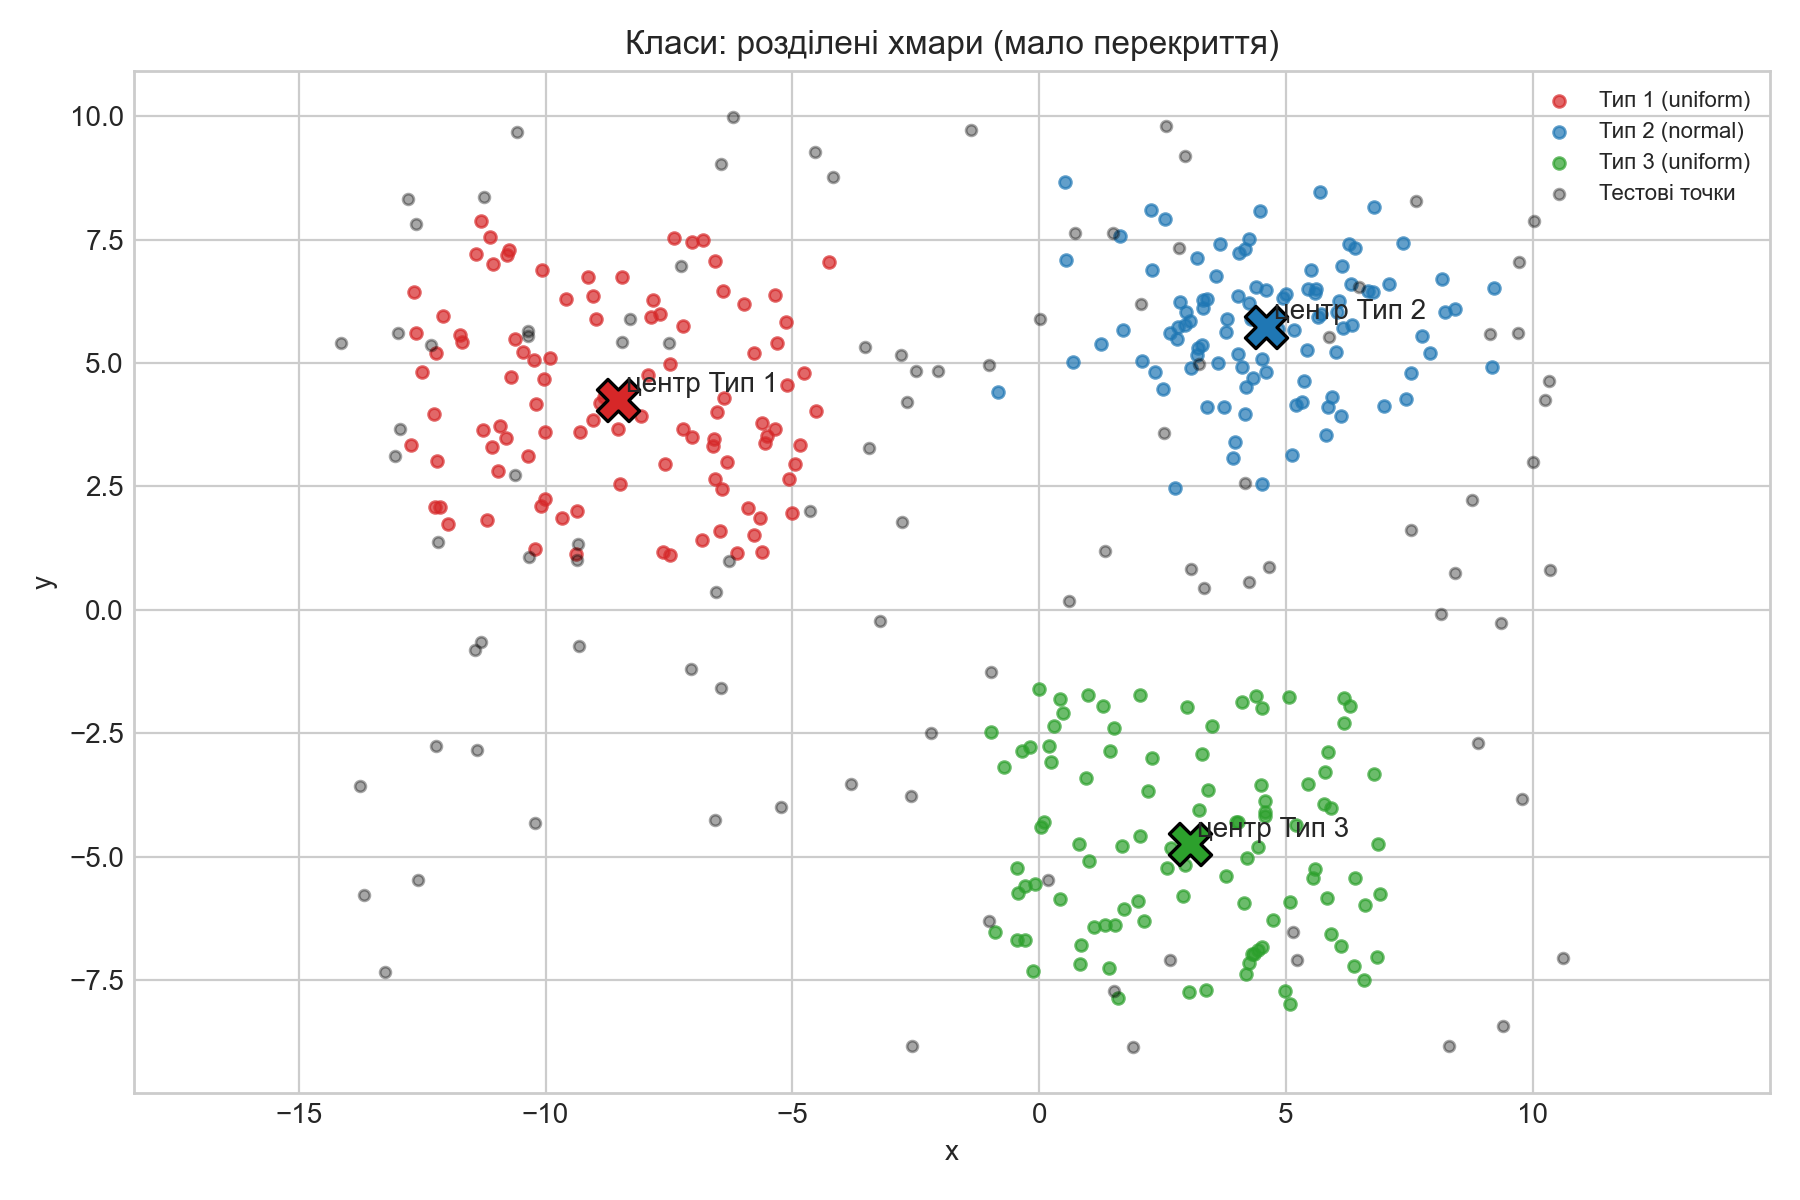
\includegraphics[width=\linewidth]{figures/lab3_scatter_separated.png}
\caption{Режим \texttt{separated}}
\end{subfigure}
\hfill
\begin{subfigure}[b]{0.48\textwidth}
\centering
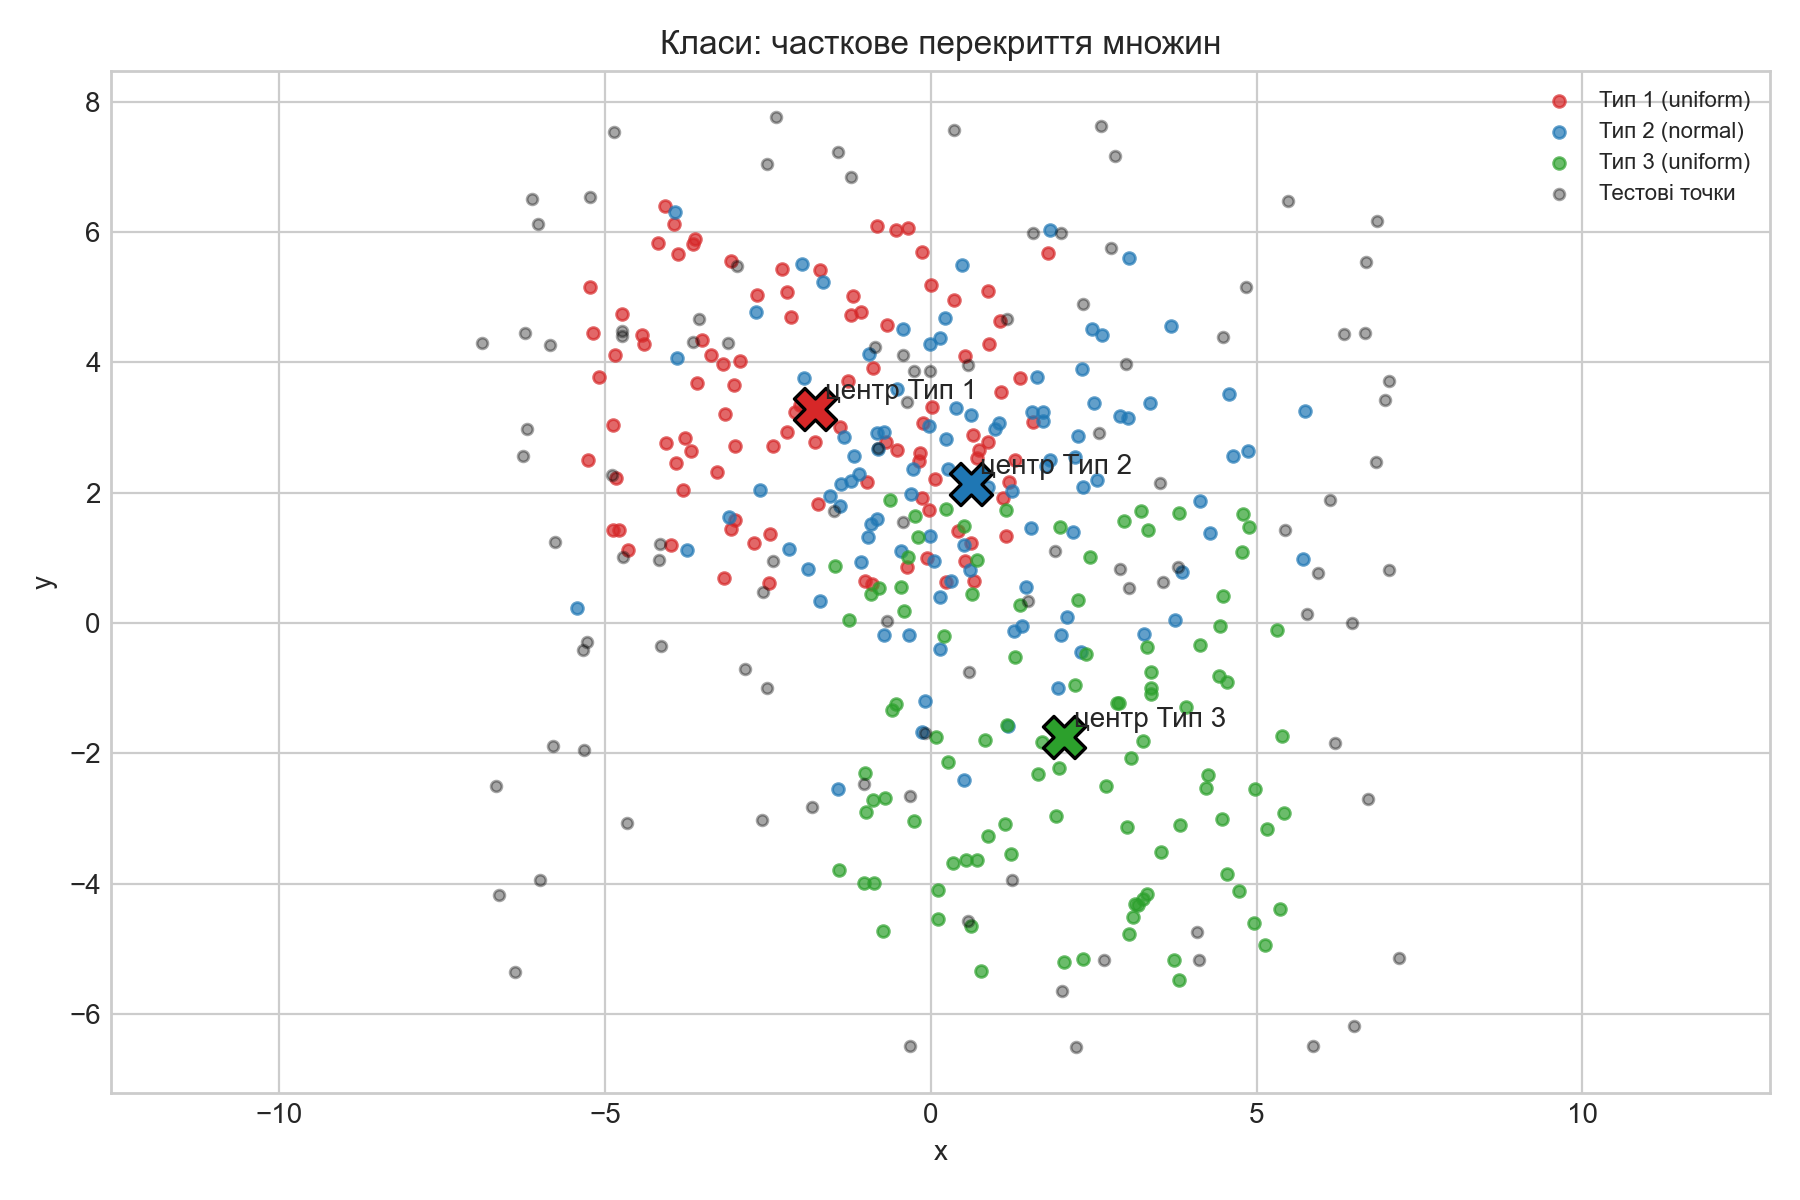
\includegraphics[width=\linewidth]{figures/lab3_scatter_overlap.png}
\caption{Режим \texttt{overlap}}
\end{subfigure}
\caption{Навчальні хмари, центроїди та тестові точки в площині $(x,y)$}
\label{fig:lab3scatter}
\end{figure}

\begin{figure}[H]
\centering
\begin{subfigure}[b]{0.48\textwidth}
\centering
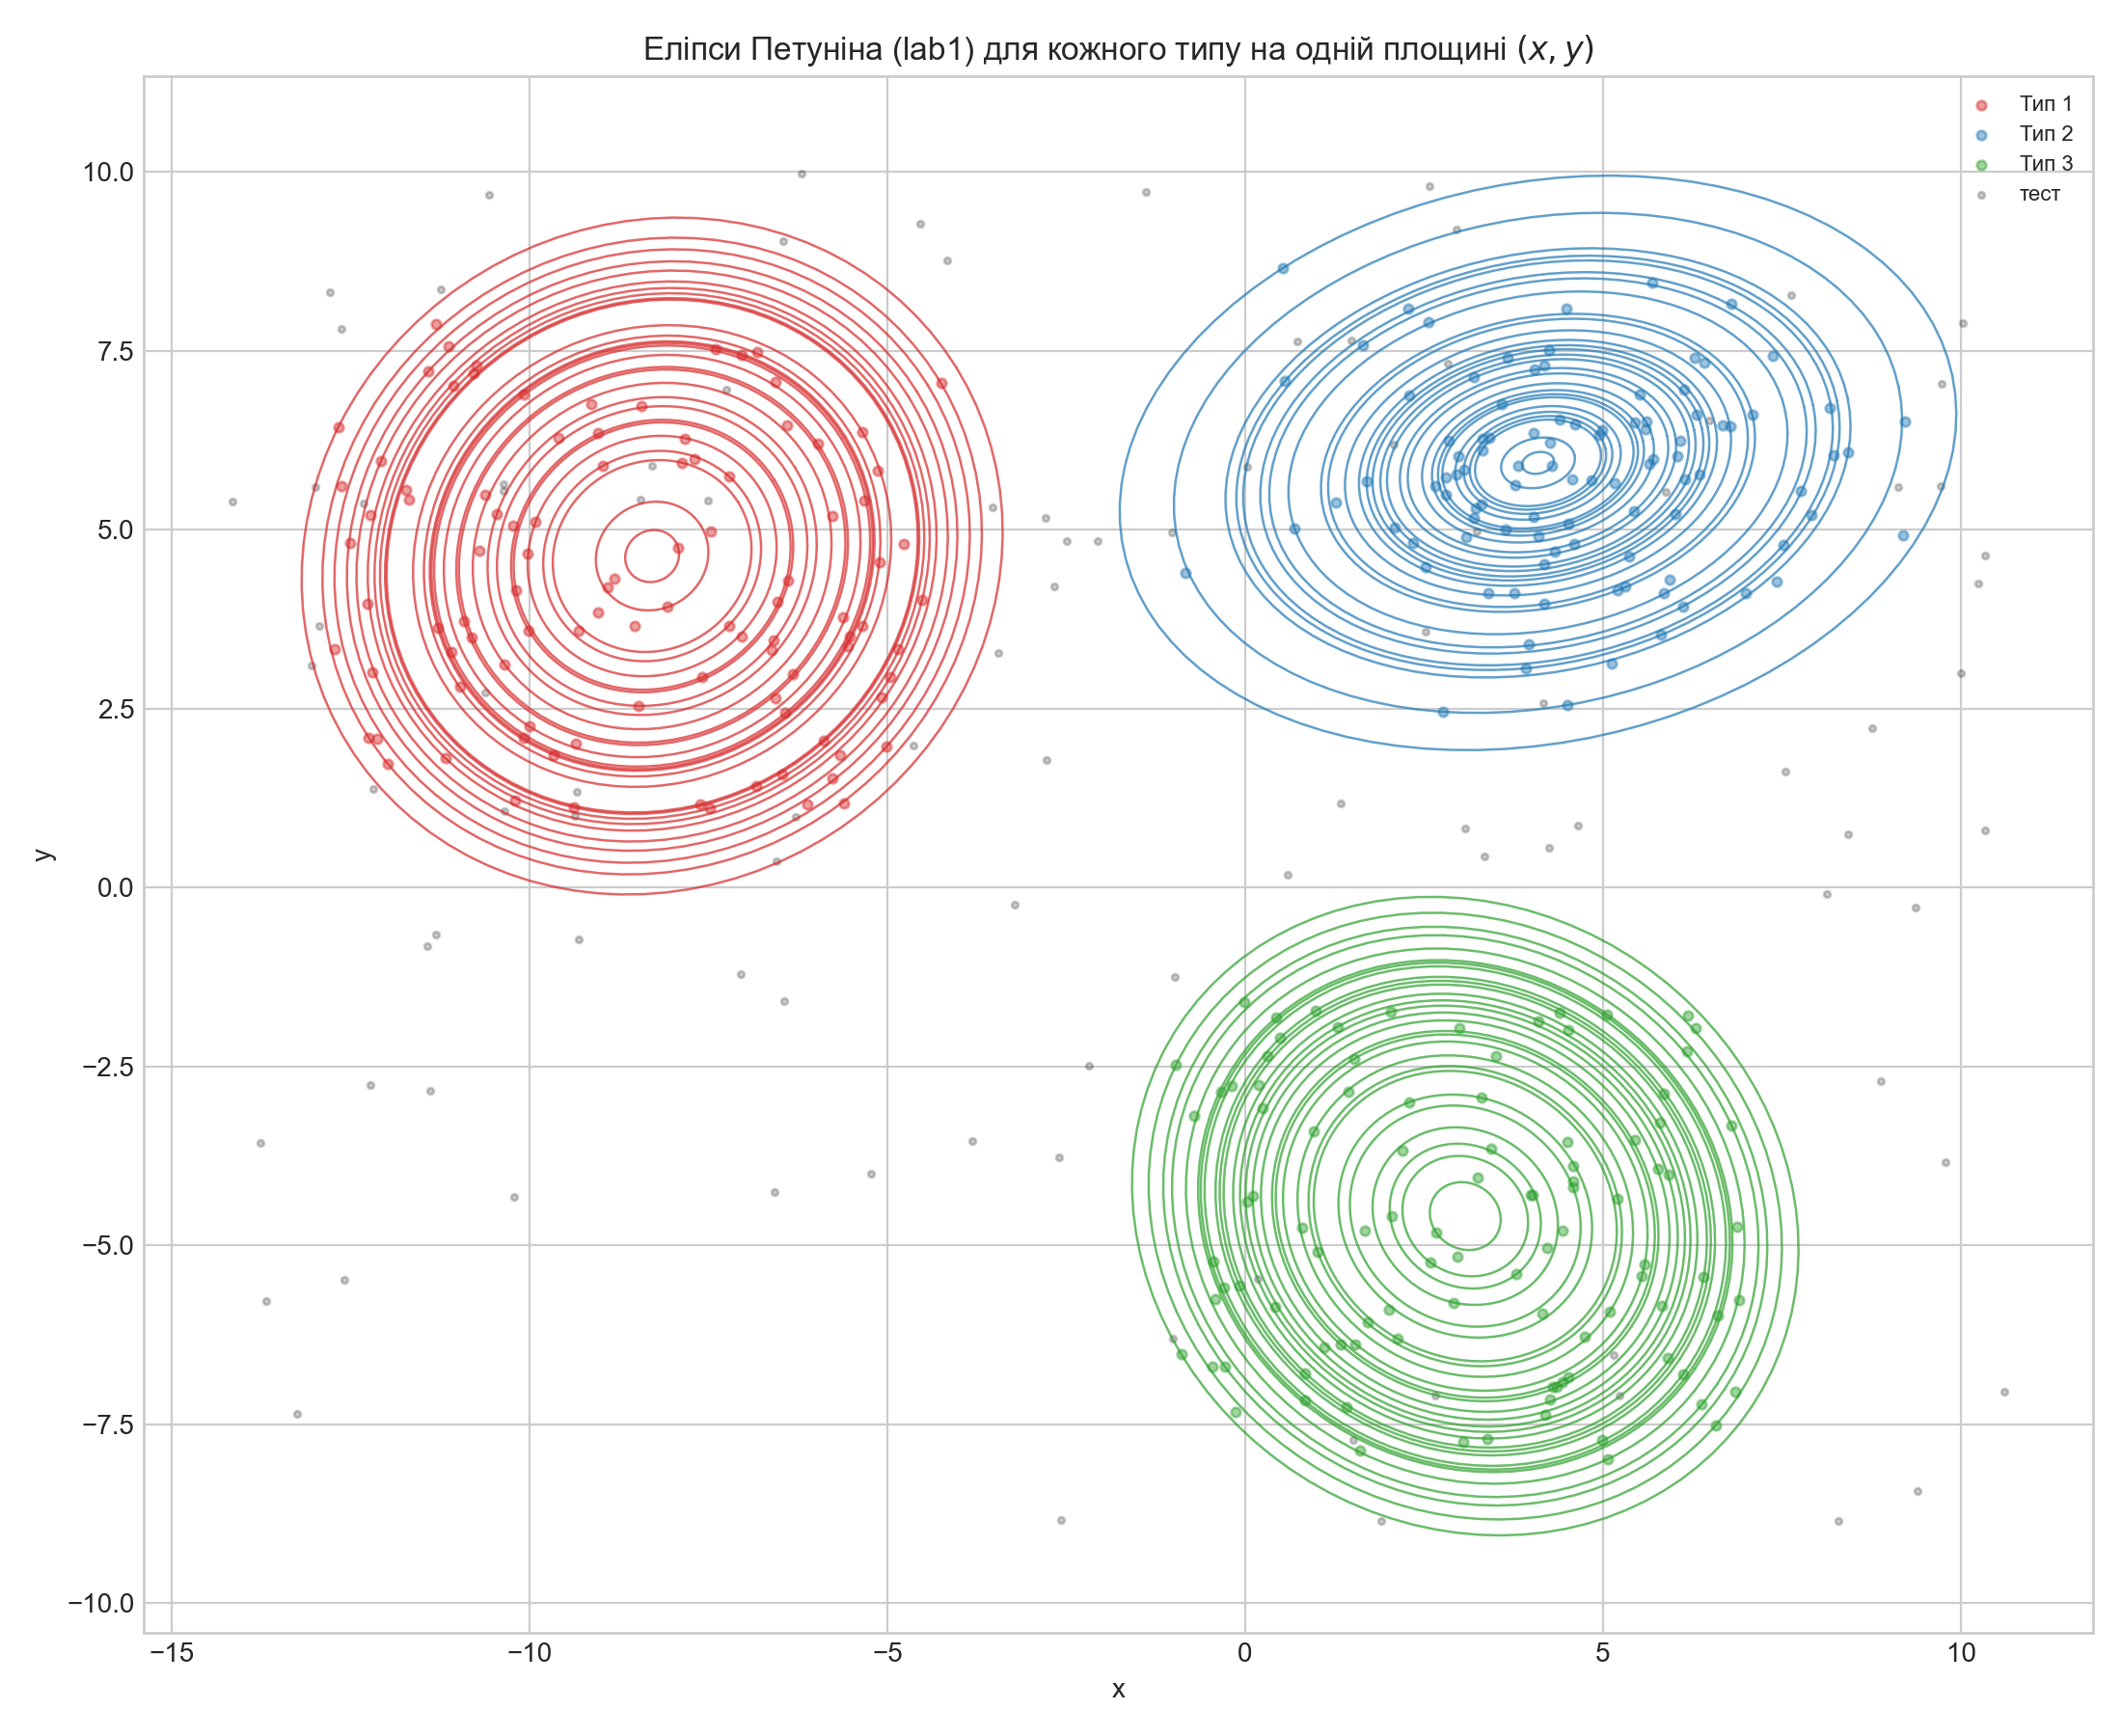
\includegraphics[width=\linewidth]{figures/lab3_petunin2d_separated.png}
\caption{\texttt{separated}}
\end{subfigure}
\hfill
\begin{subfigure}[b]{0.48\textwidth}
\centering
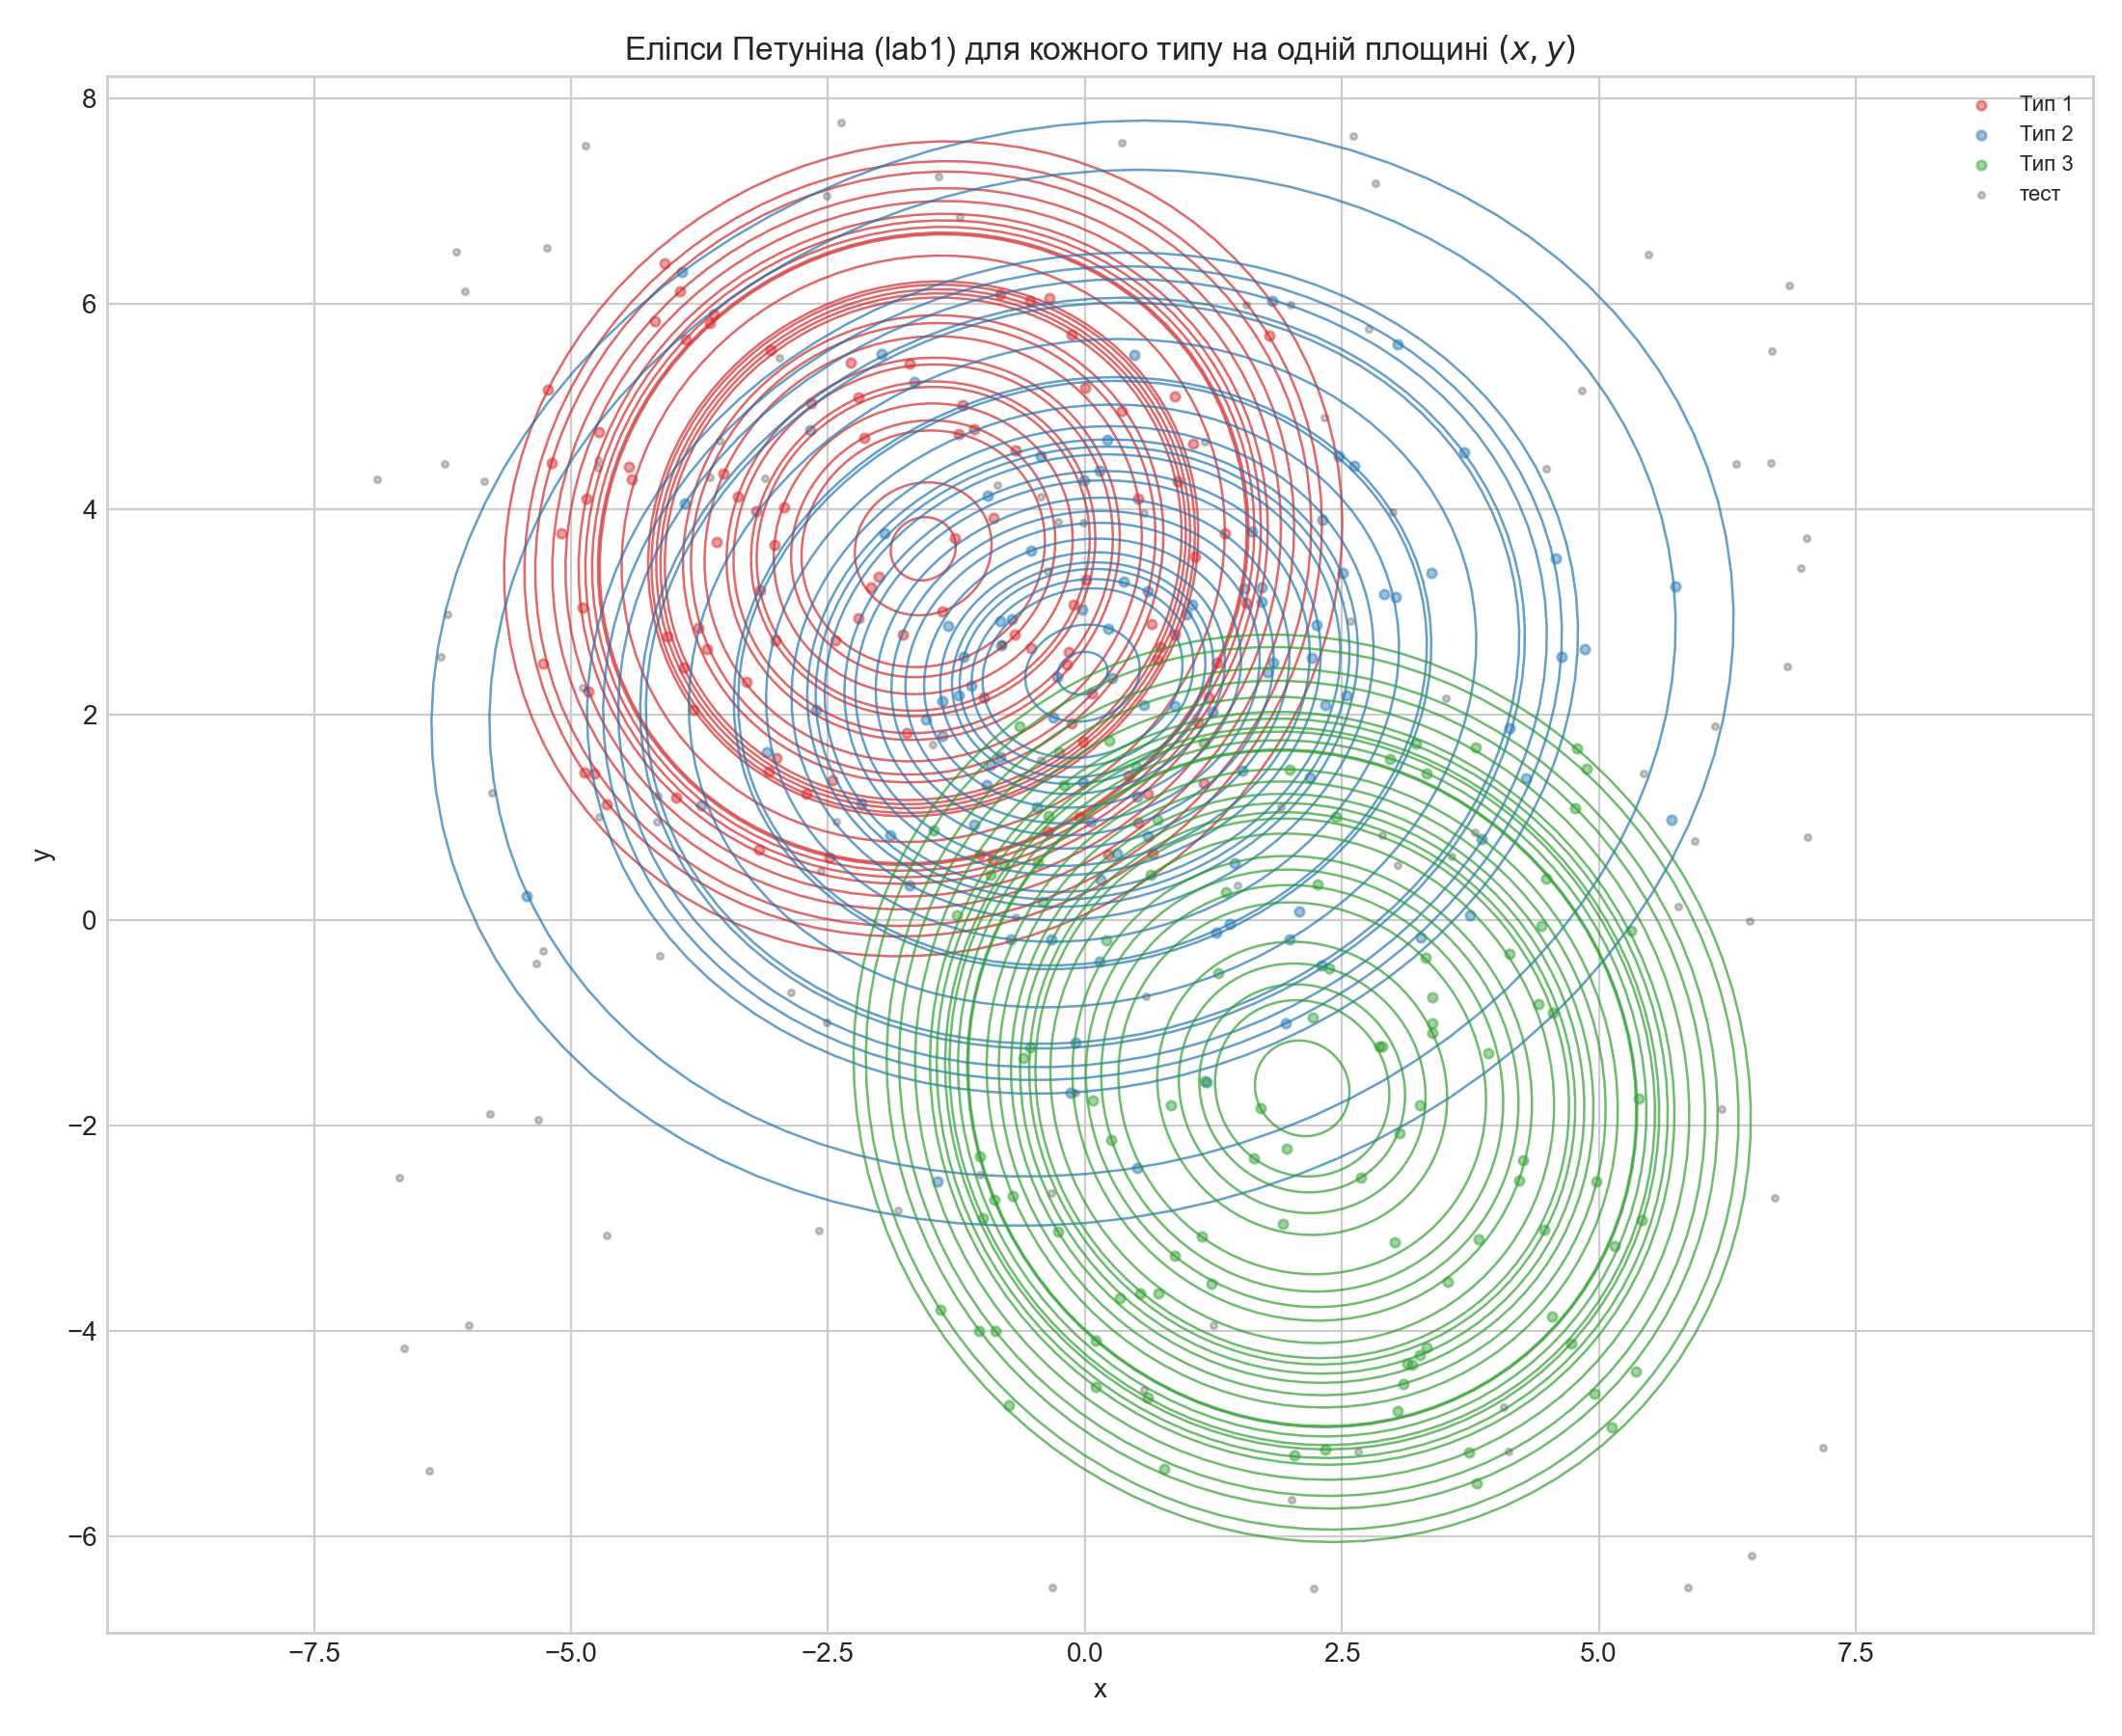
\includegraphics[width=\linewidth]{figures/lab3_petunin2d_overlap.png}
\caption{\texttt{overlap}}
\end{subfigure}
\caption{Вкладені еліпси Петуніна (2D) та тестові точки}
\label{fig:lab3pet2d}
\end{figure}

\begin{figure}[H]
\centering
\begin{subfigure}[b]{0.48\textwidth}
\centering
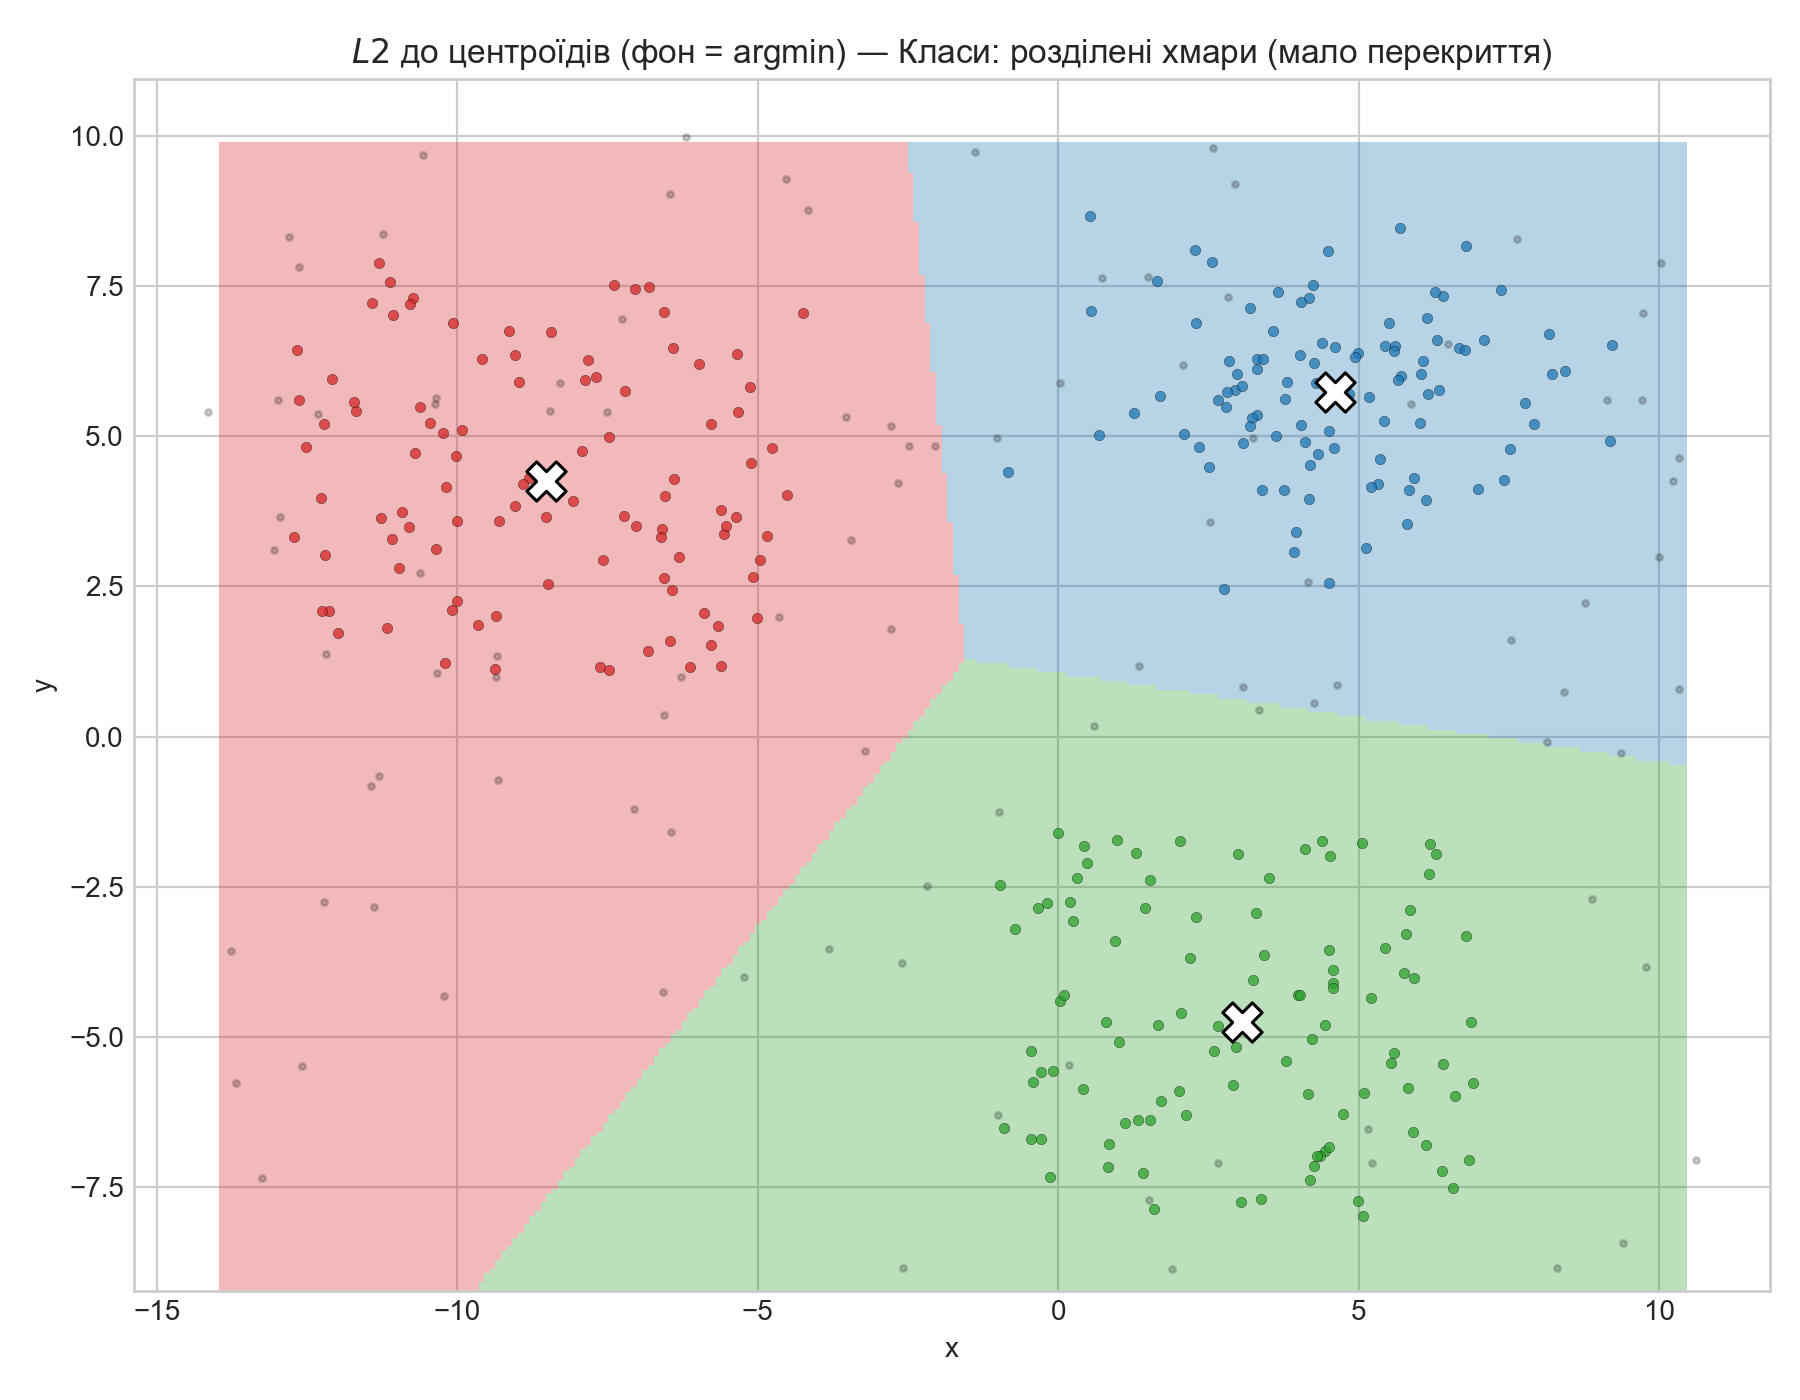
\includegraphics[width=\linewidth]{figures/lab3_l2regions_separated.png}
\caption{$L2$, \texttt{separated}}
\end{subfigure}
\hfill
\begin{subfigure}[b]{0.48\textwidth}
\centering
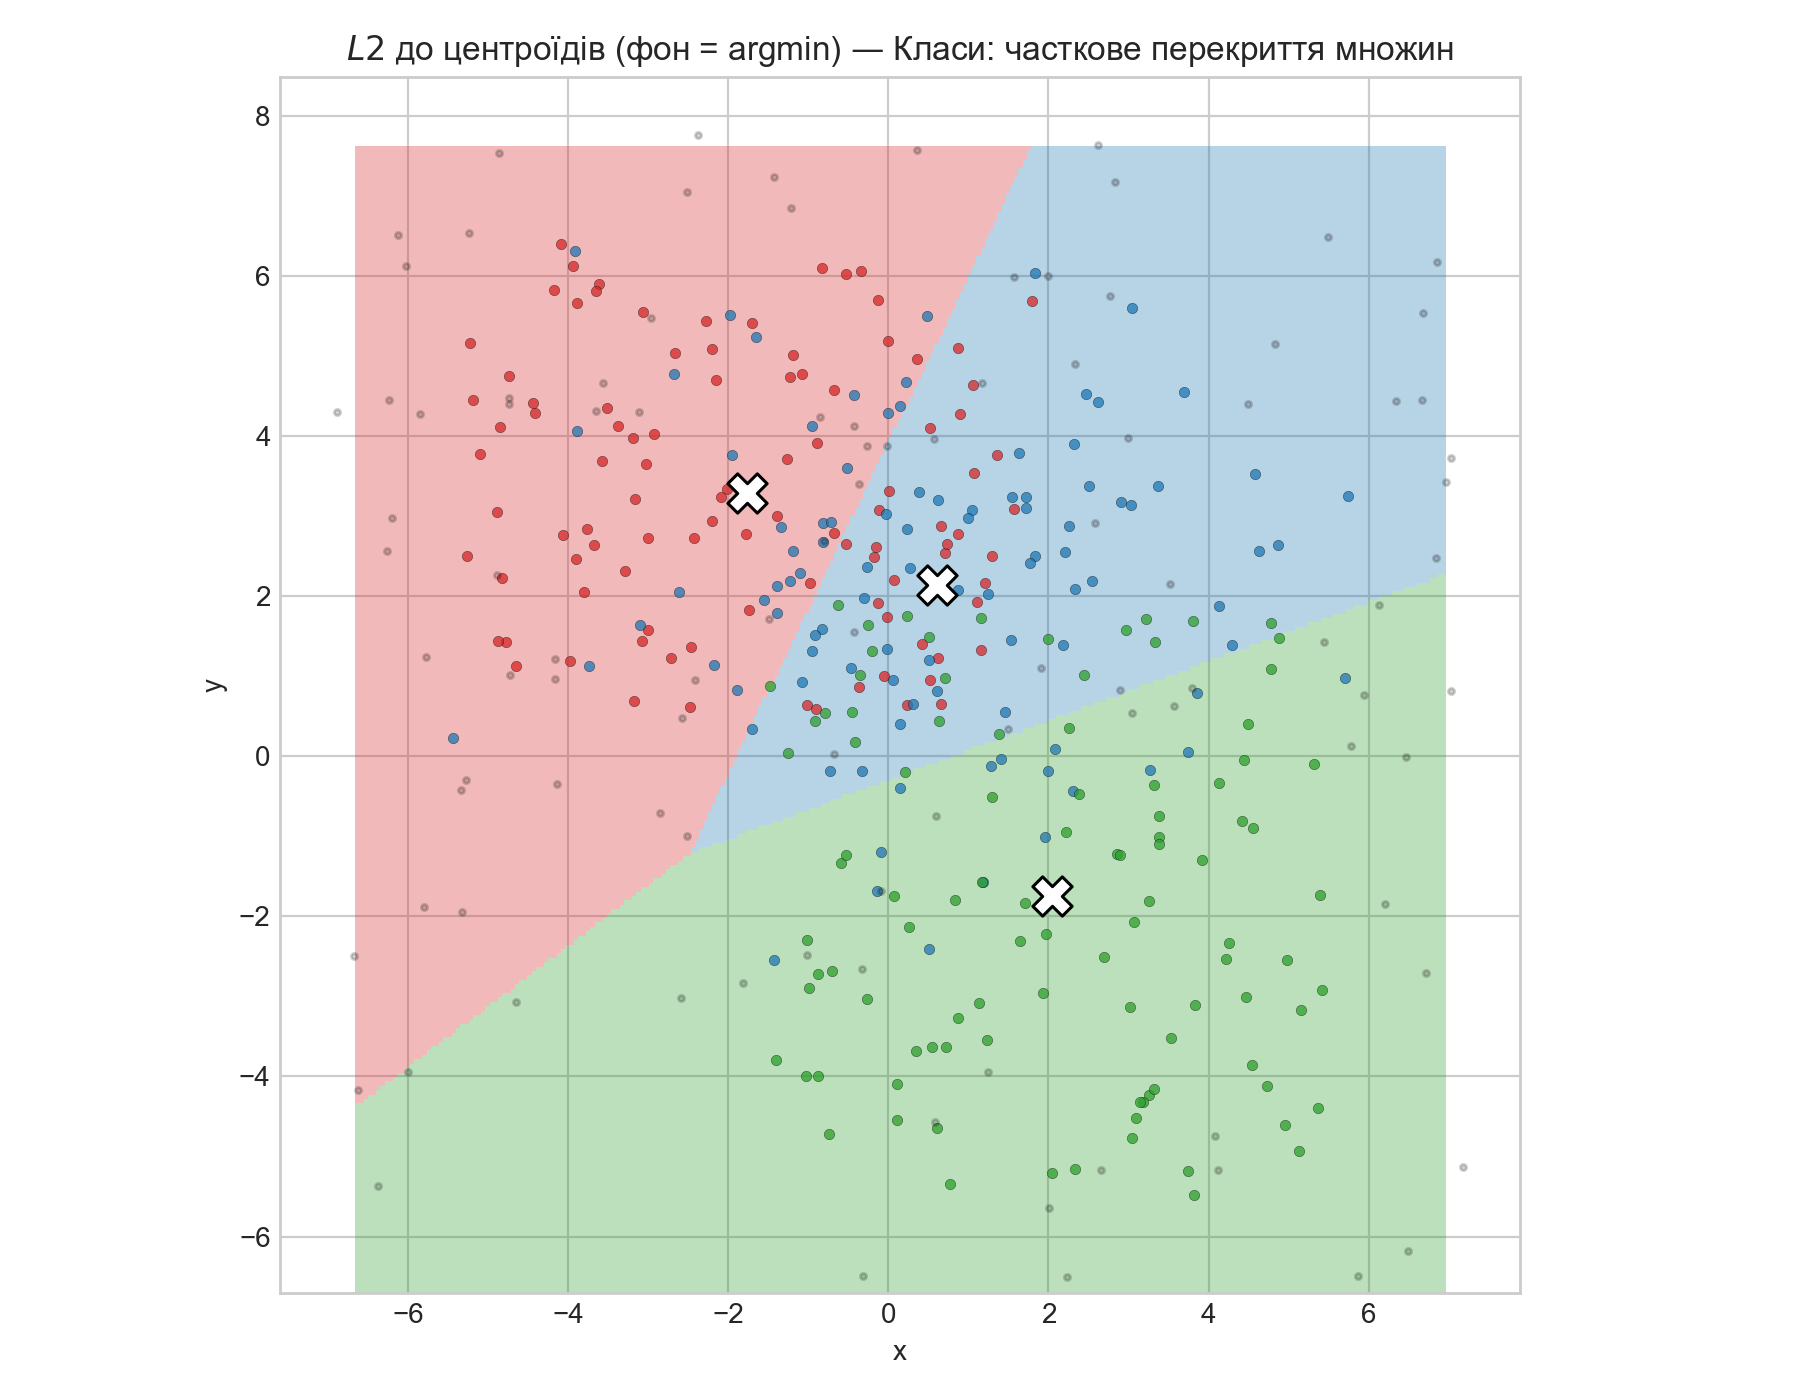
\includegraphics[width=\linewidth]{figures/lab3_l2regions_overlap.png}
\caption{$L2$, \texttt{overlap}}
\end{subfigure}
\\[0.6em]
\begin{subfigure}[b]{0.48\textwidth}
\centering
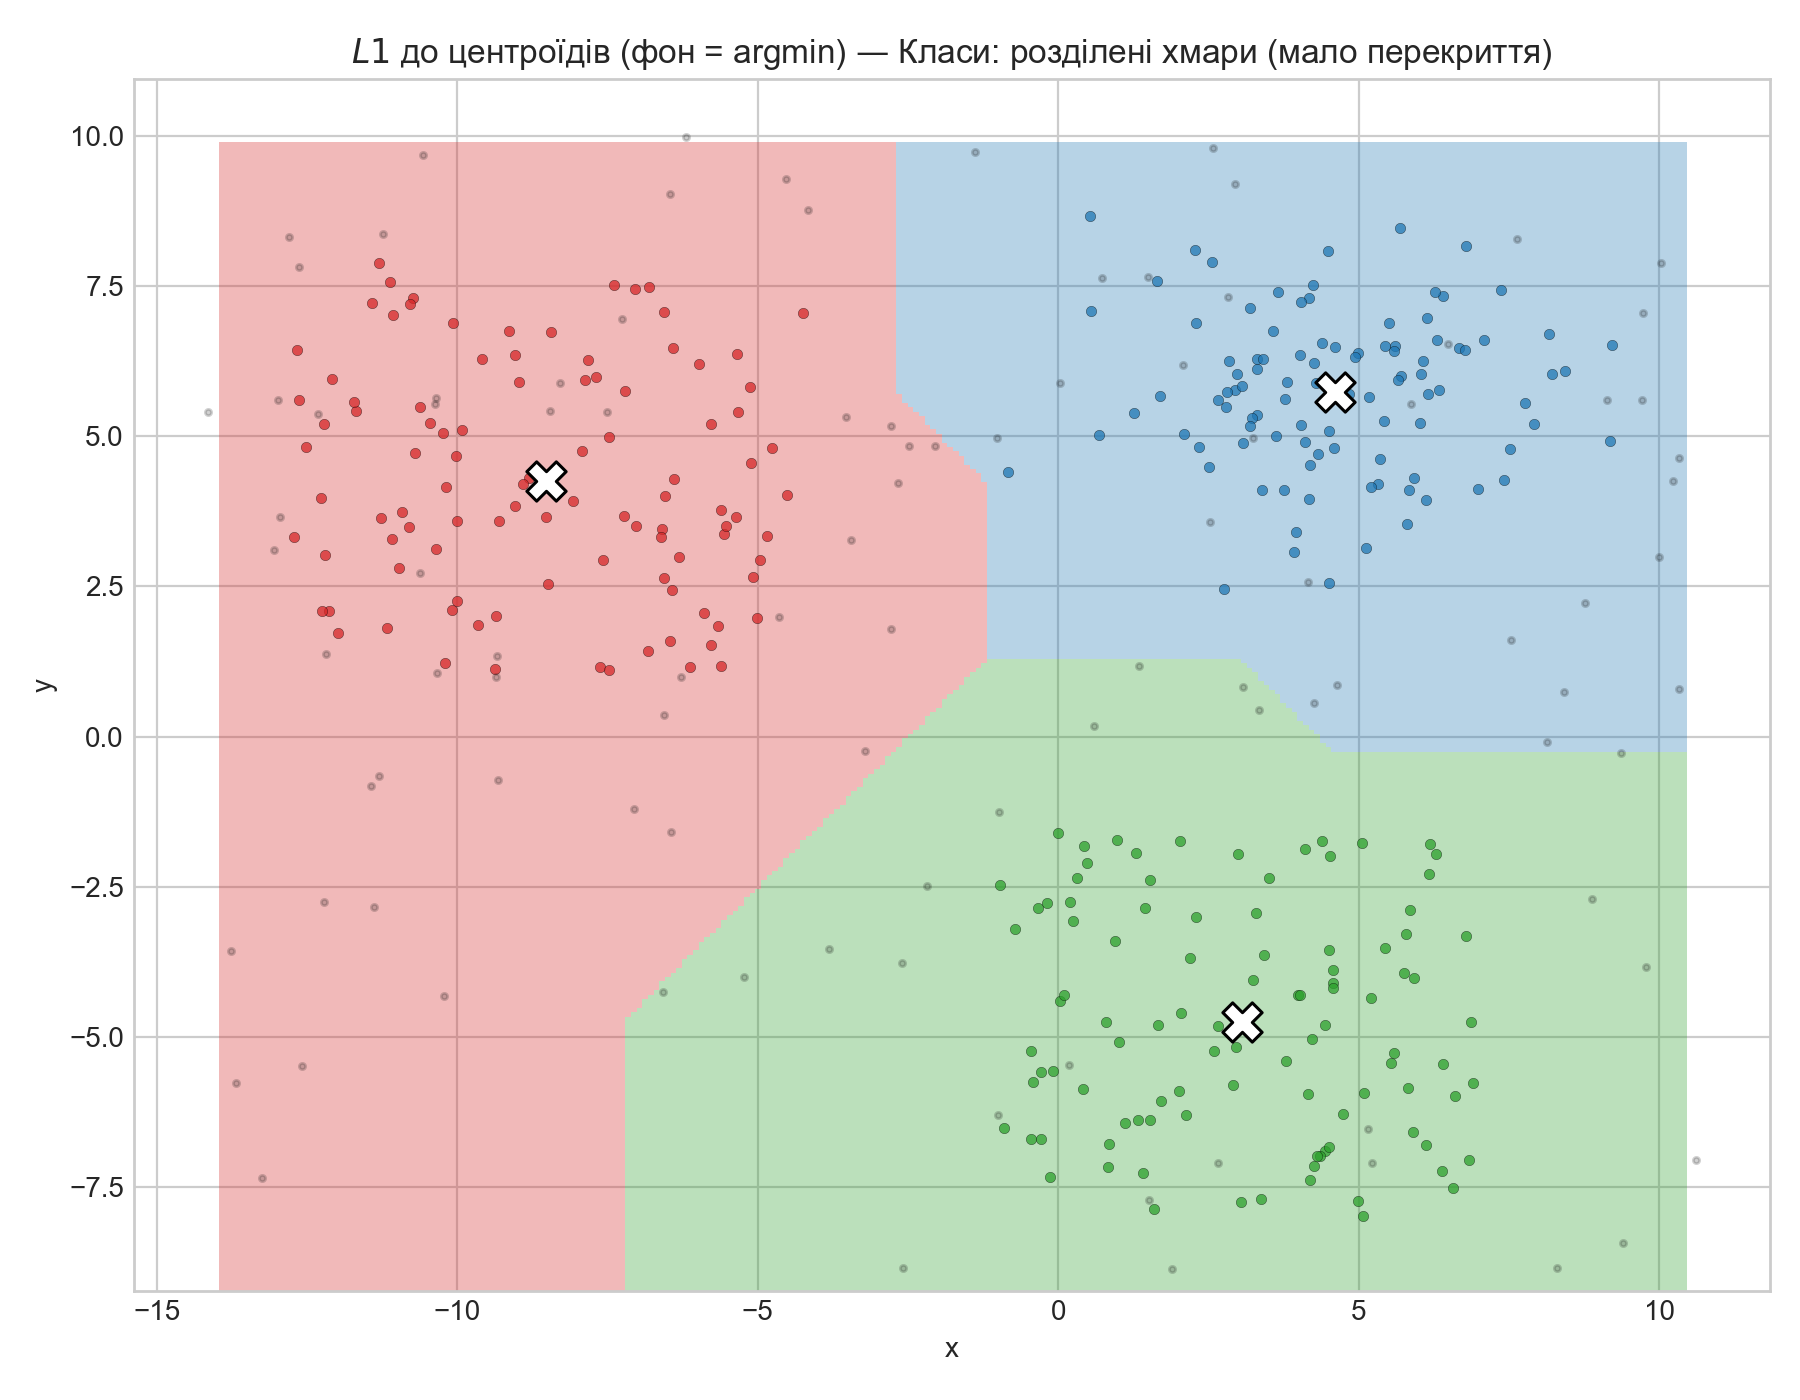
\includegraphics[width=\linewidth]{figures/lab3_l1regions_separated.png}
\caption{$L1$, \texttt{separated}}
\end{subfigure}
\hfill
\begin{subfigure}[b]{0.48\textwidth}
\centering
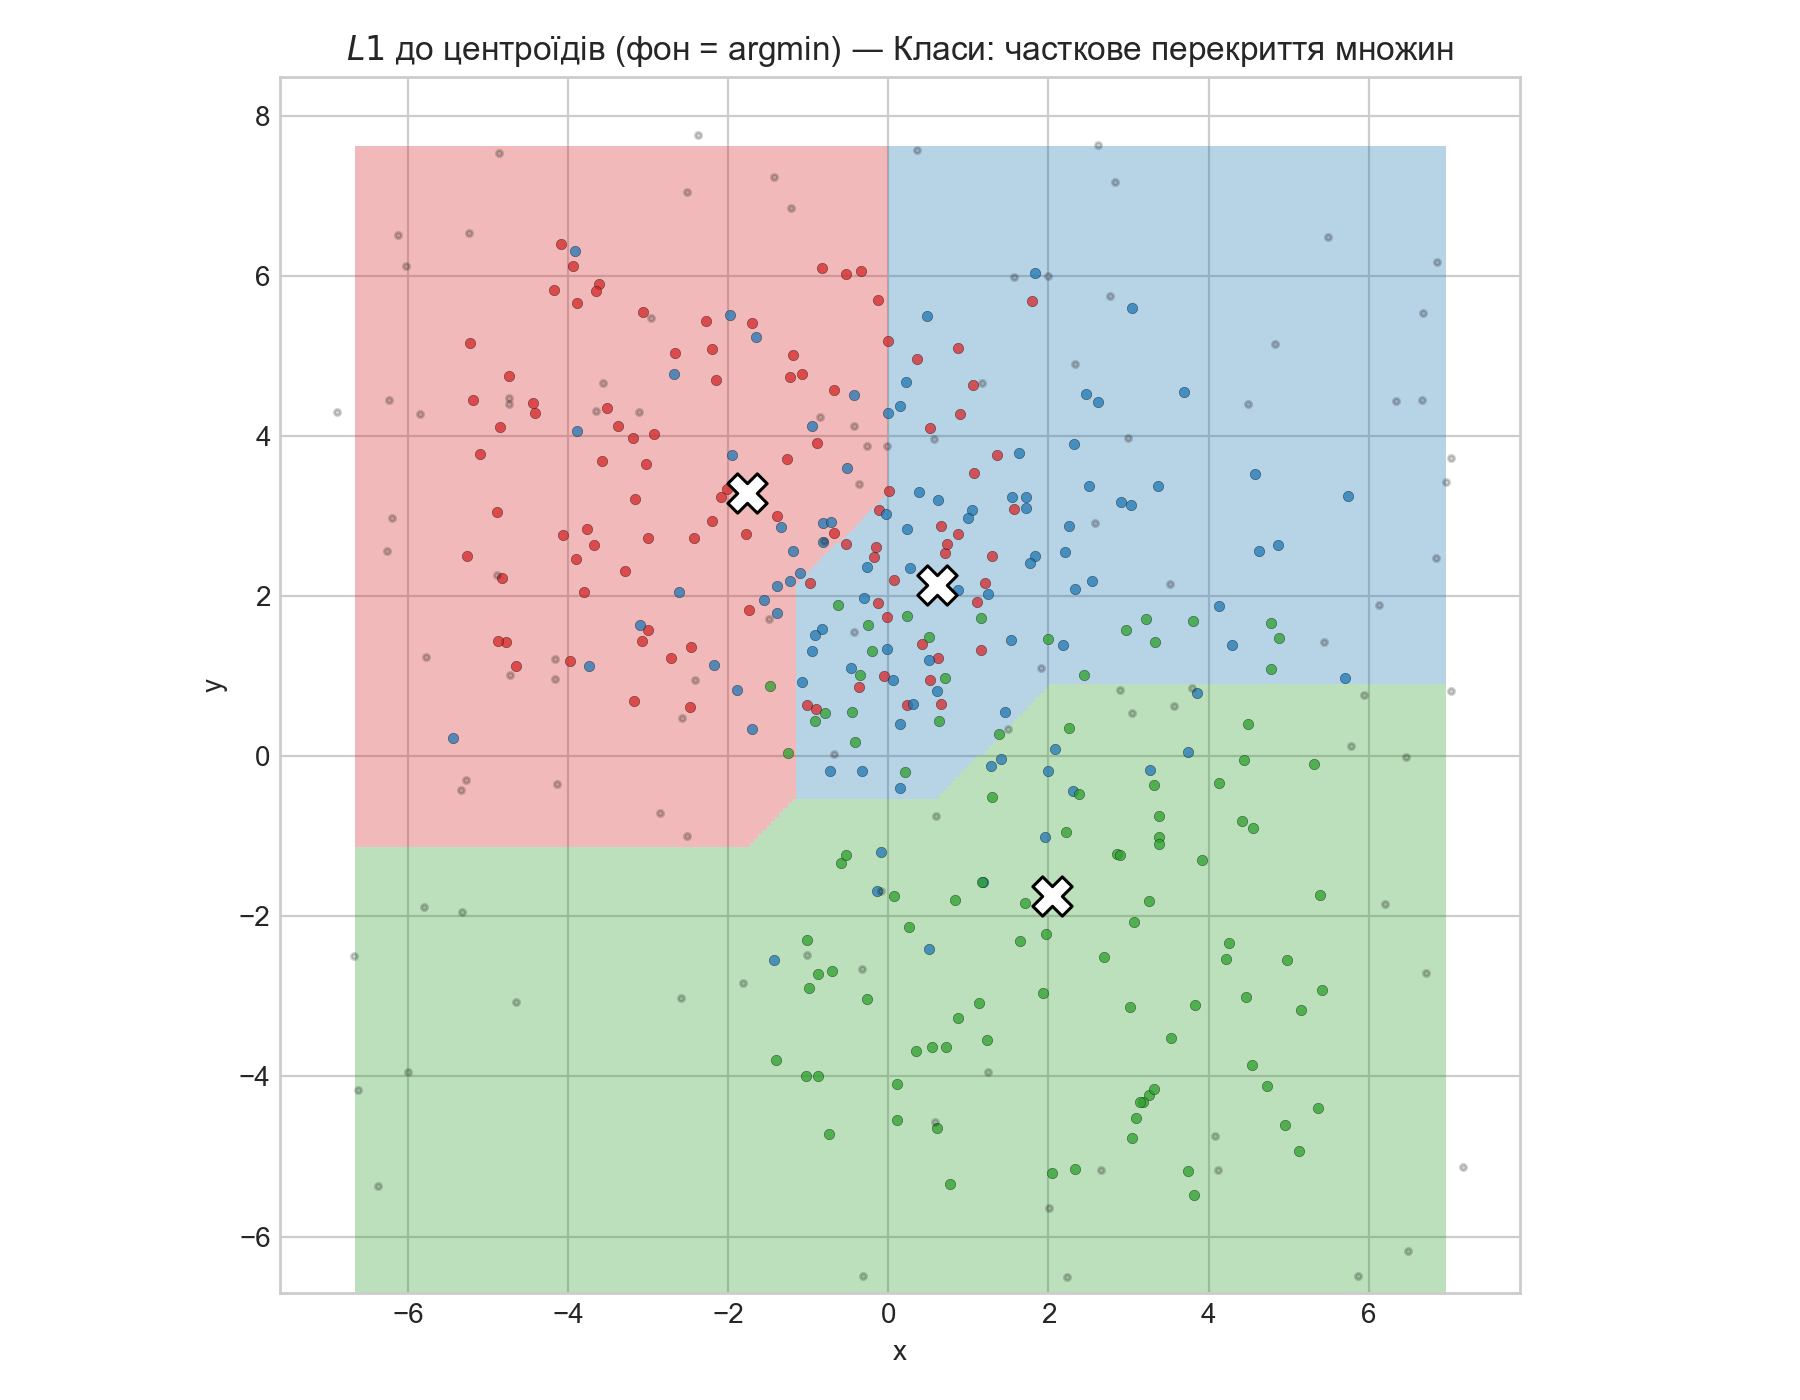
\includegraphics[width=\linewidth]{figures/lab3_l1regions_overlap.png}
\caption{$L1$, \texttt{overlap}}
\end{subfigure}
\caption{Карти рішень центроїдного класифікатора за $L2$ та $L1$ (колір фону --- клас за argmin на сітці)}
\label{fig:lab3l2l1}
\end{figure}

\begin{figure}[H]
\centering
\begin{subfigure}[b]{0.48\textwidth}
\centering
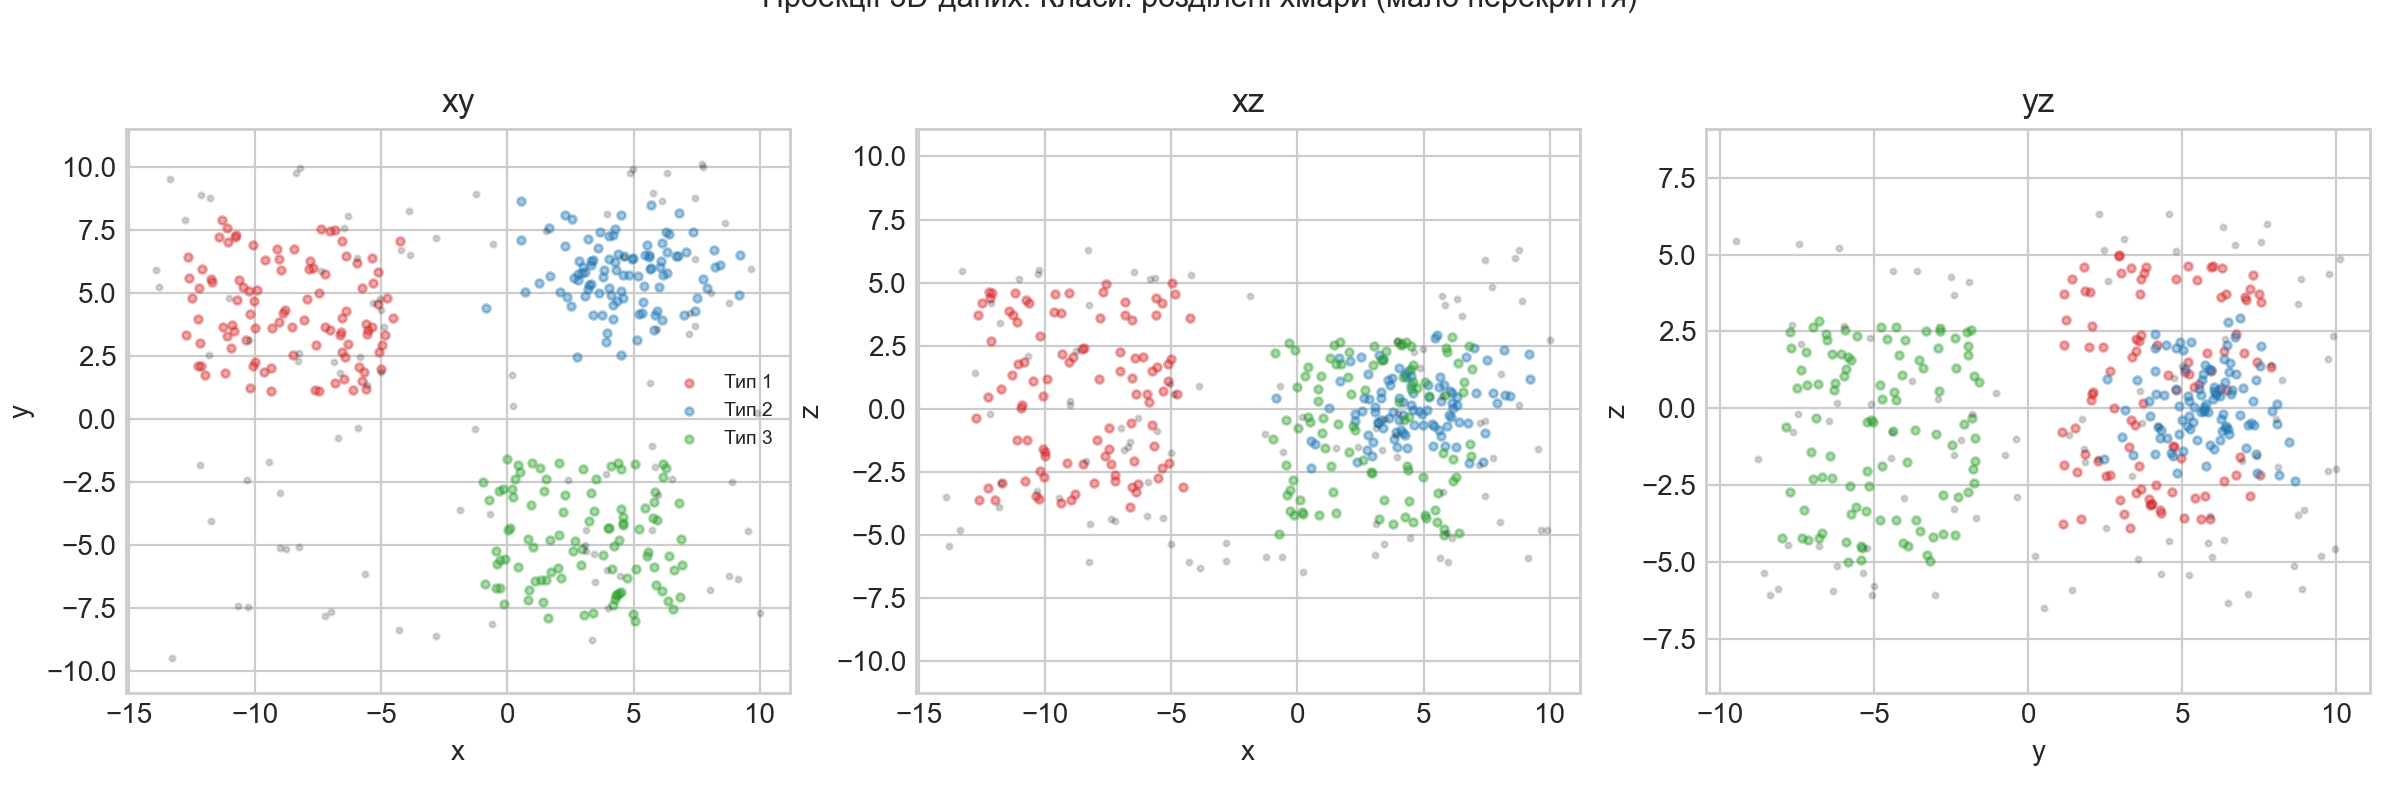
\includegraphics[width=\linewidth]{figures/lab3_projections_separated.png}
\caption{\texttt{separated}}
\end{subfigure}
\hfill
\begin{subfigure}[b]{0.48\textwidth}
\centering
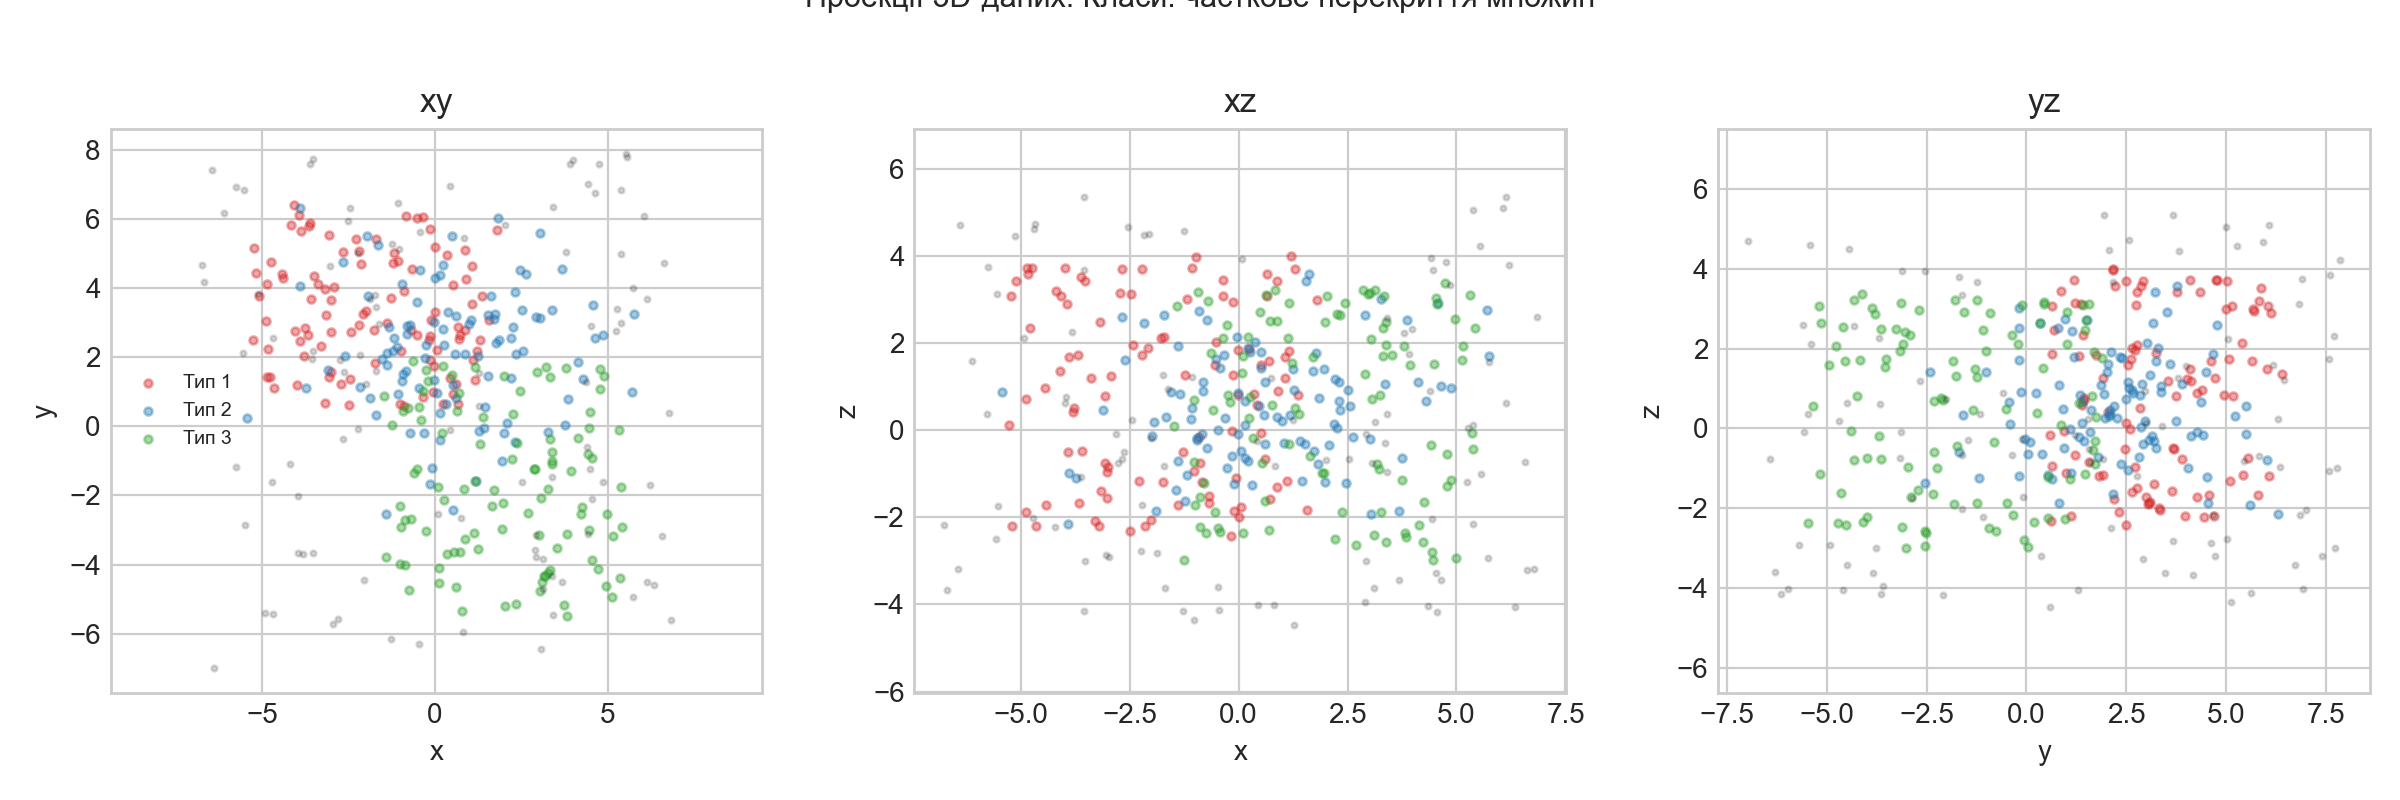
\includegraphics[width=\linewidth]{figures/lab3_projections_overlap.png}
\caption{\texttt{overlap}}
\end{subfigure}
\caption{Проекції 3D-даних на площини $xy$, $xz$, $yz$}
\label{fig:lab3proj}
\end{figure}

\begin{figure}[H]
\centering
\begin{subfigure}[b]{0.48\textwidth}
\centering
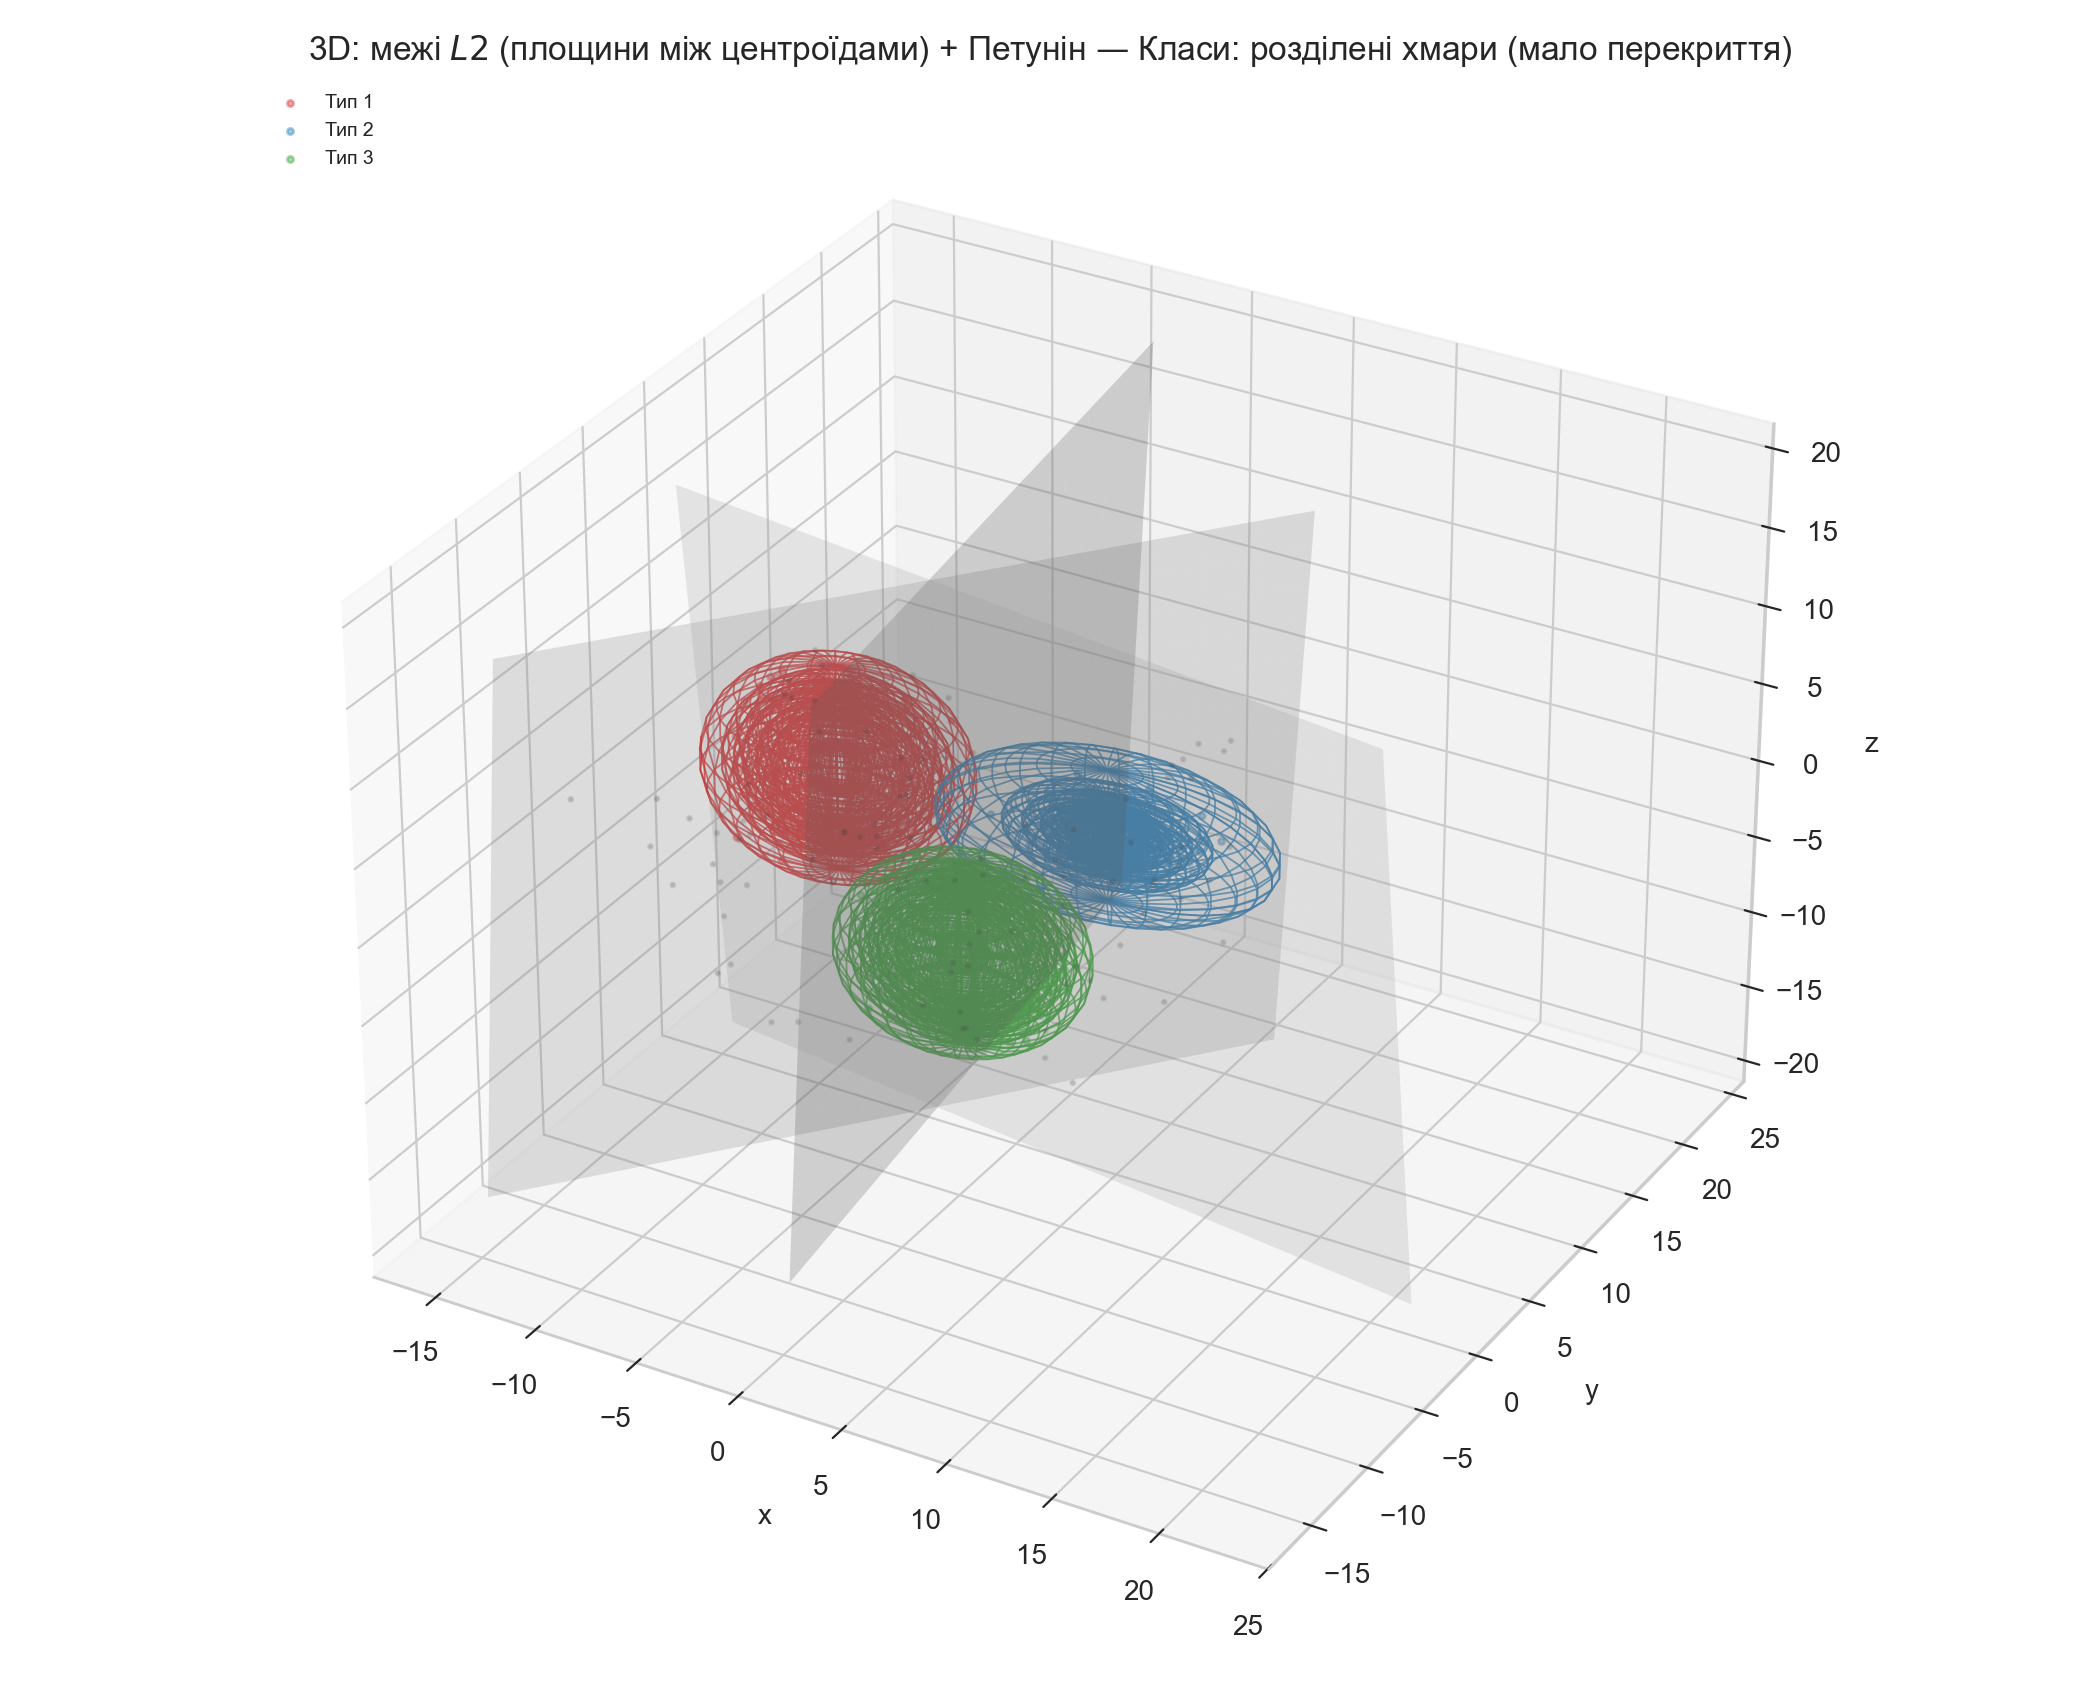
\includegraphics[width=\linewidth]{figures/lab3_3d_l2_pet_separated.png}
\caption{\texttt{separated}}
\end{subfigure}
\hfill
\begin{subfigure}[b]{0.48\textwidth}
\centering
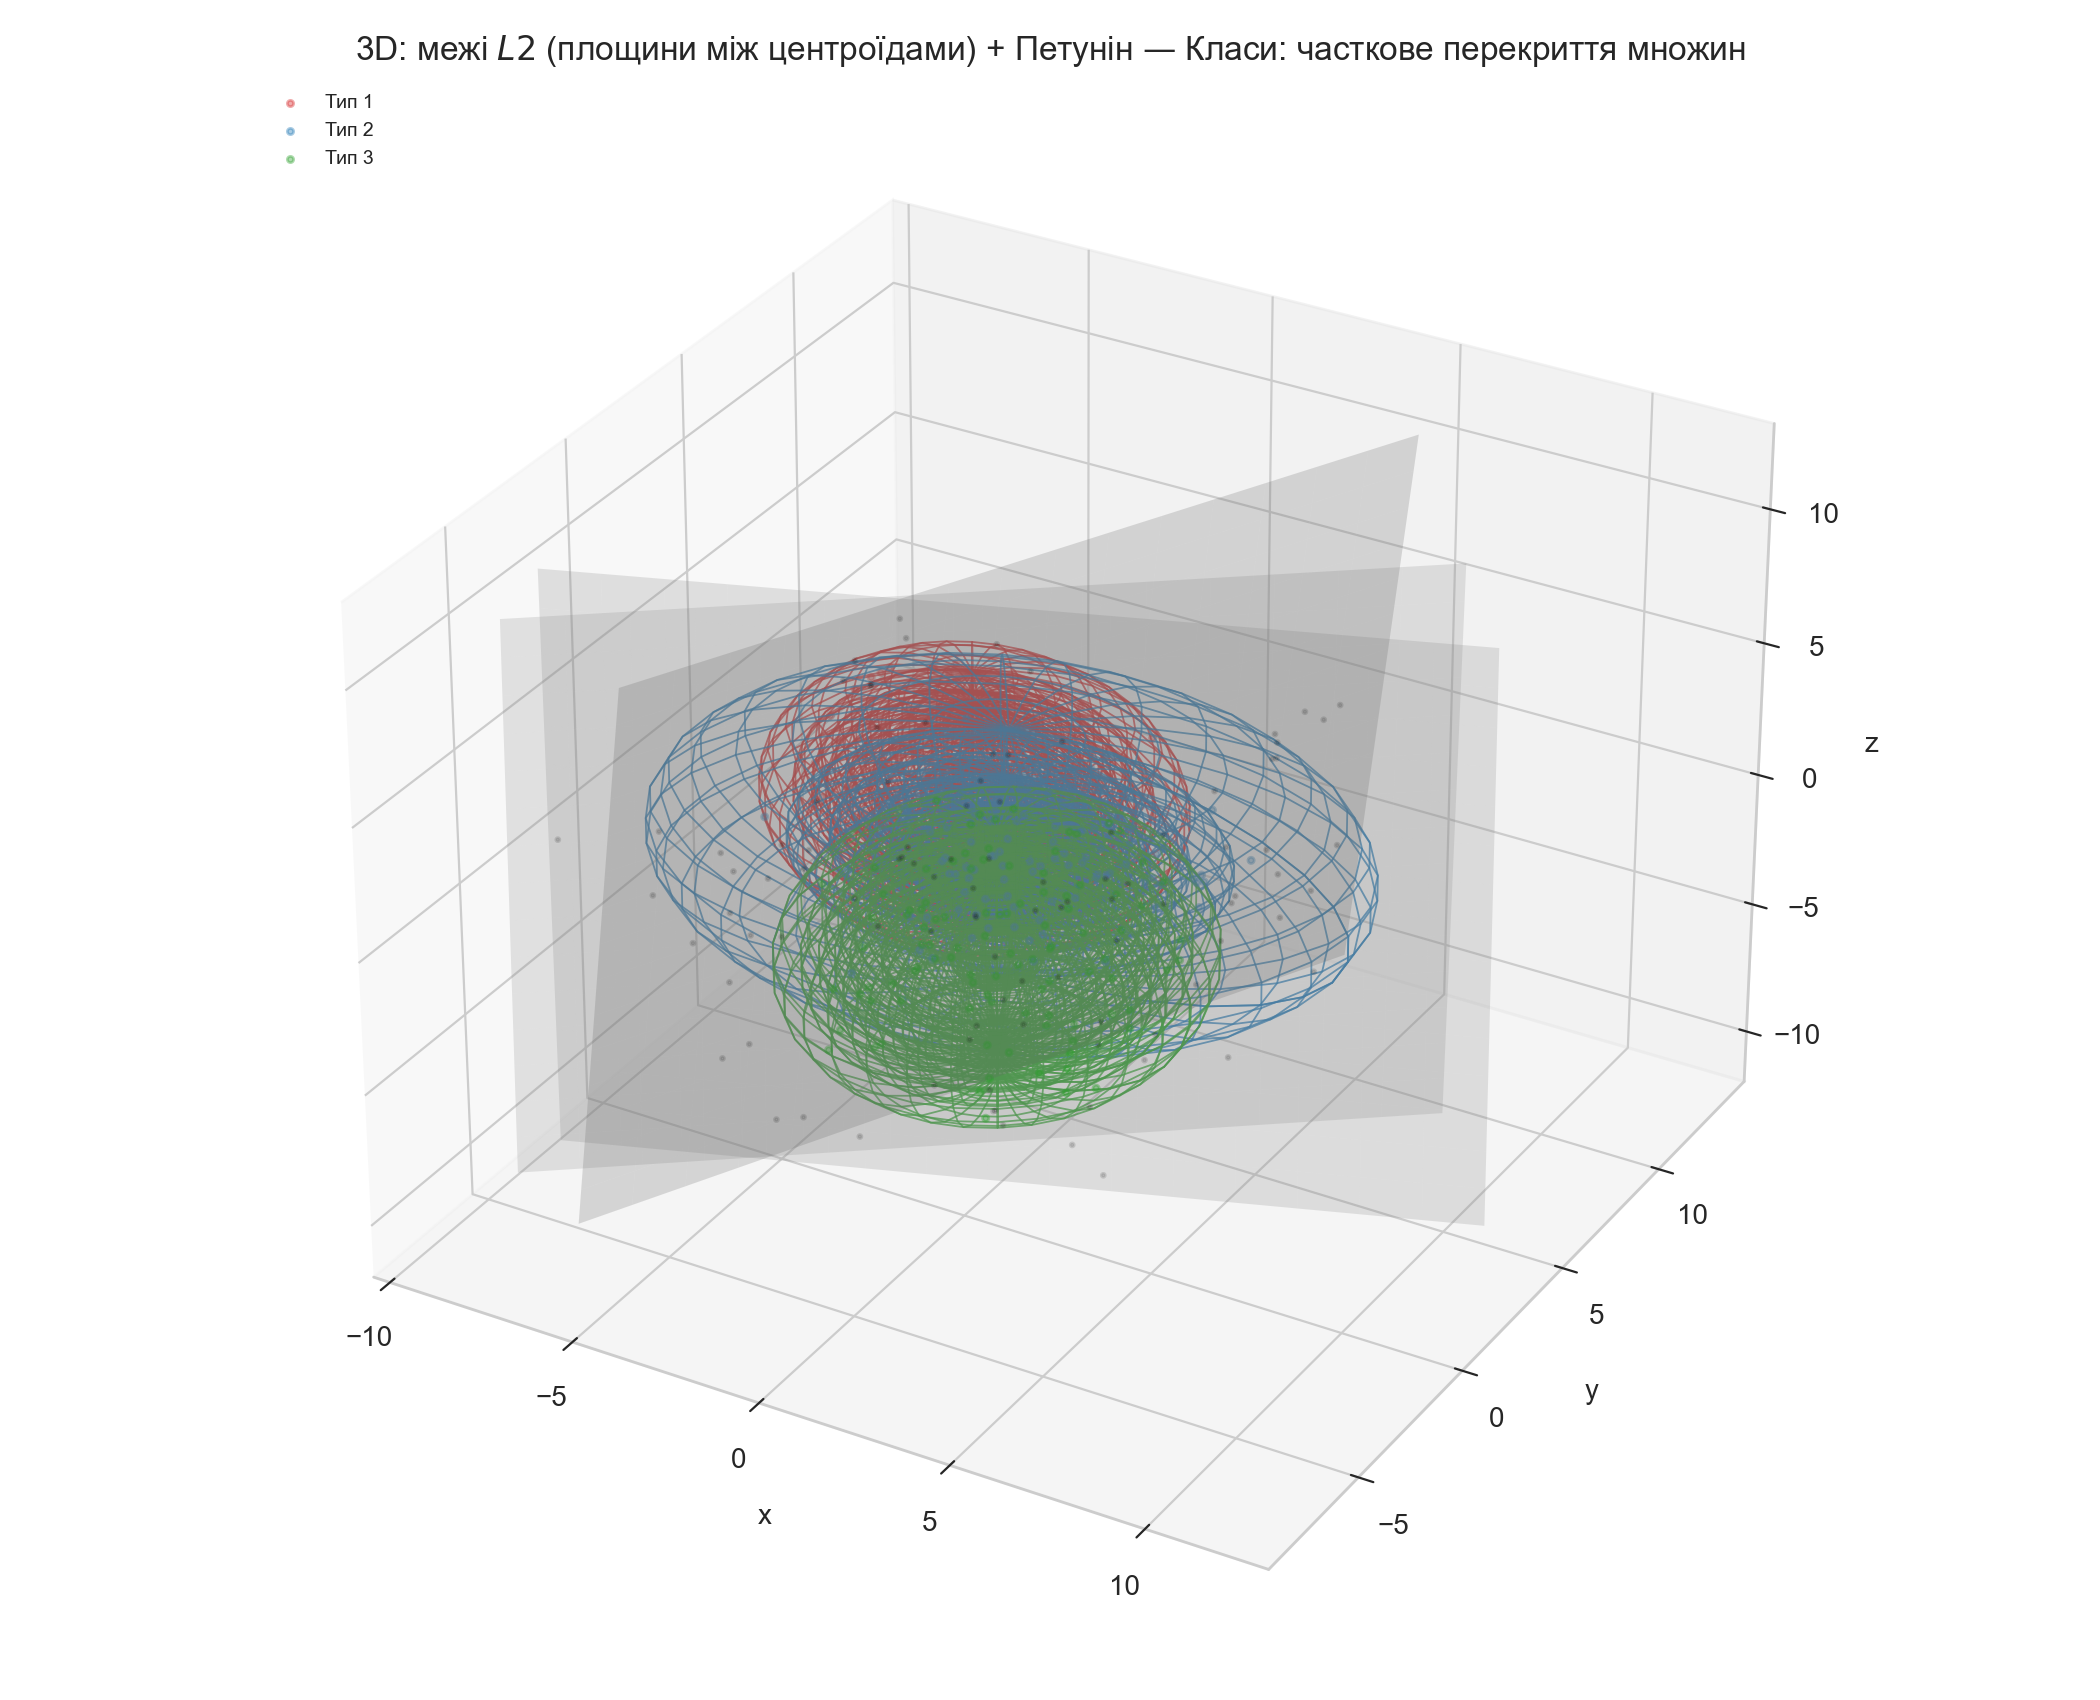
\includegraphics[width=\linewidth]{figures/lab3_3d_l2_pet_overlap.png}
\caption{\texttt{overlap}}
\end{subfigure}
\caption{3D: площини рівної $L2$-відстані між центроїдами та каркас еліпсоїдів Петуніна}
\label{fig:lab33d}
\end{figure}

%================ ВИСНОВКИ ================
\section{Висновки}
\begin{enumerate}
    \item Реалізовано класифікацію трьох типів за центроїдними метриками $L2$ та $L1$ у $(x,y)$, а також за еліпсами та еліпсоїдами Петуніна у~2D та~3D при узгодженій генерації координати~$z$.
    \item Порівняно два режими генерації (\texttt{separated} та \texttt{overlap}): за таблицею~\ref{tab:lab3mismatch} видно, що при перекритті множин зростає кількість розбіжностей між $L2$ і Петуніним (2D та 3D), тобто геометрія правила суттєво впливає на рішення в спірних зонах.
    \item Метрика $L1$ дає ромбоподібні рівні відстані в $(x,y)$ і може відрізнятися від $L2$ на прикордонних точках; еліпси Петуніна відображають форму навчальної хмари, а не лише положення центру.
    \item Рисунки~\ref{fig:lab3scatter}--\ref{fig:lab33d} узгоджені з таблицею~\ref{tab:lab3mismatch}: видно карти $L2$/$L1$, вкладені еліпси та тривимірні межі $L2$ разом із каркасом еліпсоїдів.
    \item Обмеження підходу: центроїдні евристики та еліпси Петуніна не задають байєсівський оптимум для перекривних класів; результати демонстраційні й залежать від вибору областей генерації та випадкового seed.
\end{enumerate}

\end{document}
